%==============================================================================
%  ARTIGO CIENTIFICO - Concepcao e Design de Projeto Transformador
%  Engenharia Mecanica - PUCPR
%  Layout adaptado a partir do template Word fornecido:
%    - A4, margens ~2 cm, Times New Roman
%    - Cabecalho em todas as paginas
%    - Titulo / autores / afiliacao / resumo / palavras-chave em 1 coluna
%    - Corpo do artigo em 2 colunas
%    - Citacoes numericas estilo [1]
%==============================================================================
\documentclass[a4paper,10pt,twocolumn]{article}

\usepackage[utf8]{inputenc}
\usepackage[T1]{fontenc}
\usepackage[brazilian,provide=*]{babel}  % 'provide=*' carrega o pt-BR via babel moderno
\usepackage{mathptmx}        % Times New Roman (texto + matematica)
\usepackage{amsmath}
\usepackage{amssymb}
\usepackage{siunitx}

% ----- Geometria da pagina (espelha o template: A4, margens ~2 cm) ----------
\usepackage{geometry}
\geometry{a4paper, left=2cm, right=2cm, top=2.3cm, bottom=1.5cm,
          headsep=0.5cm, columnsep=0.6cm}

\usepackage{setspace}
\usepackage{indentfirst}
\usepackage{graphicx}
\usepackage{float}
\usepackage{booktabs}
\usepackage{array}
\usepackage{tabularx}
\usepackage{ragged2e}
\usepackage[font=small,labelfont=bf]{caption}

% ----- Cabecalho em todas as paginas (igual ao template) --------------------
\usepackage{fancyhdr}
\pagestyle{fancy}
\fancyhf{}
\renewcommand{\headrulewidth}{0.4pt}
\fancyhead[C]{\footnotesize\itshape Concepção e Design de Projeto
              Transformador -- Engenharia Mecânica -- 1\textsuperscript{o}
              Semestre 2026}
\fancyfoot[C]{\thepage}

% ----- Espacamentos das secoes proximos do template -------------------------
\usepackage{titlesec}
\titleformat{\section}{\normalfont\bfseries}{\thesection.}{0.5em}{\MakeUppercase}
\titleformat{\subsection}{\normalfont\bfseries}{\thesubsection}{0.5em}{}
\titleformat{\subsubsection}{\normalfont\itshape}{\thesubsubsection}{0.5em}{}
\titlespacing*{\section}{0pt}{1.2em}{0.6em}
\titlespacing*{\subsection}{0pt}{0.8em}{0.4em}

\usepackage[hidelinks]{hyperref}

% ----- Estilo das citacoes numericas [1] e referencias ----------------------
% (requer o pacote, ja padrao em distribuicoes TeX)
\usepackage[numbers,square,sort&compress]{natbib}
\setlength{\bibsep}{0pt}

\setlength{\parindent}{1.25em}
\setlength{\columnsep}{0.6cm}

\begin{document}

%==============================================================================
%  CABECALHO
%==============================================================================
\twocolumn[
  \begin{@twocolumnfalse}
  \begin{center}
    {\LARGE Vibrometria óptica aplicada para medição de vibrações
     em testes dinâmicos de bancada\par}
    \vspace{1em}
    {\large Vinicius Andrade Trento\textsuperscript{1} e
     Prof. Helio Emmendoerfer Junior\textsuperscript{2}\par}
    \vspace{0.6em}
    {\itshape Pontifícia Universidade Católica do Paraná -- Engenharia Mecânica\par}
    {\itshape vinicius.trento@pucpr.br \qquad helio.emmendoerfer@pucpr.br\par}
  \end{center}
  \vspace{0.5em}
  \hrule
  \vspace{0.8em}

  % ----- RESUMO -----
  {\noindent\bfseries\itshape Resumo}
  \par\vspace{0.3em}
  {\small\justifying\noindent
  Texto de até 250 palavras. O resumo deve ser conciso e direto, incluindo
  brevemente o objetivo do trabalho, os principais resultados e as conclusões
  mais importantes. (Substituir por seu resumo.) Este trabalho explora e valida
  a aplicação de metodologias não intrusivas de vibrometria óptica para medição
  de vibrações em testes dinâmicos de bancada, utilizando câmeras de vídeo
  convencionais e estimativa de movimento baseada em fase com filtros de Gabor,
  buscando uma alternativa de baixo custo e \textit{full-field} aos métodos
  tradicionais por contato.\par}

  \vspace{0.6em}
  {\noindent\bfseries\itshape Palavras-Chave}{\itshape: vibrometria óptica;
  estimativa de movimento baseada em fase; análise modal; SHM;
  processamento de imagens.\par}

  \vspace{1.2em}
  \hrule
  \vspace{1.2em}
  \end{@twocolumnfalse}
]

%==============================================================================
%  CORPO DO ARTIGO 
%==============================================================================

\section{Introdução}

Os acelerômetros são os dispositivos mais difundidos para a medição de vibrações nos setores automotivo, aeroespacial e industrial \cite{Anna2026}. Eles operam através da detecção de forças estáticas contínuas ou de vibrações e movimentos dinâmicos, sendo capazes de capturar fenômenos que variam desde impactos e oscilações comuns até eventos sísmicos. Dependendo do tipo de elemento sensível utilizado, esses sensores são classificados em piezorresistivos, capacitivos, piezoelétricos ou ressonantes \cite{PiezoAccelerometer2023}. A Figura \ref{fig:acelerometro_dewesoft} apresenta um esquema representativo de um acelerômetro de compressão piezoelétrico, um dos tipos mais comuns utilizados em aplicações industriais para medição de altas frequências.

\begin{figure}[htbp]
    \centering
    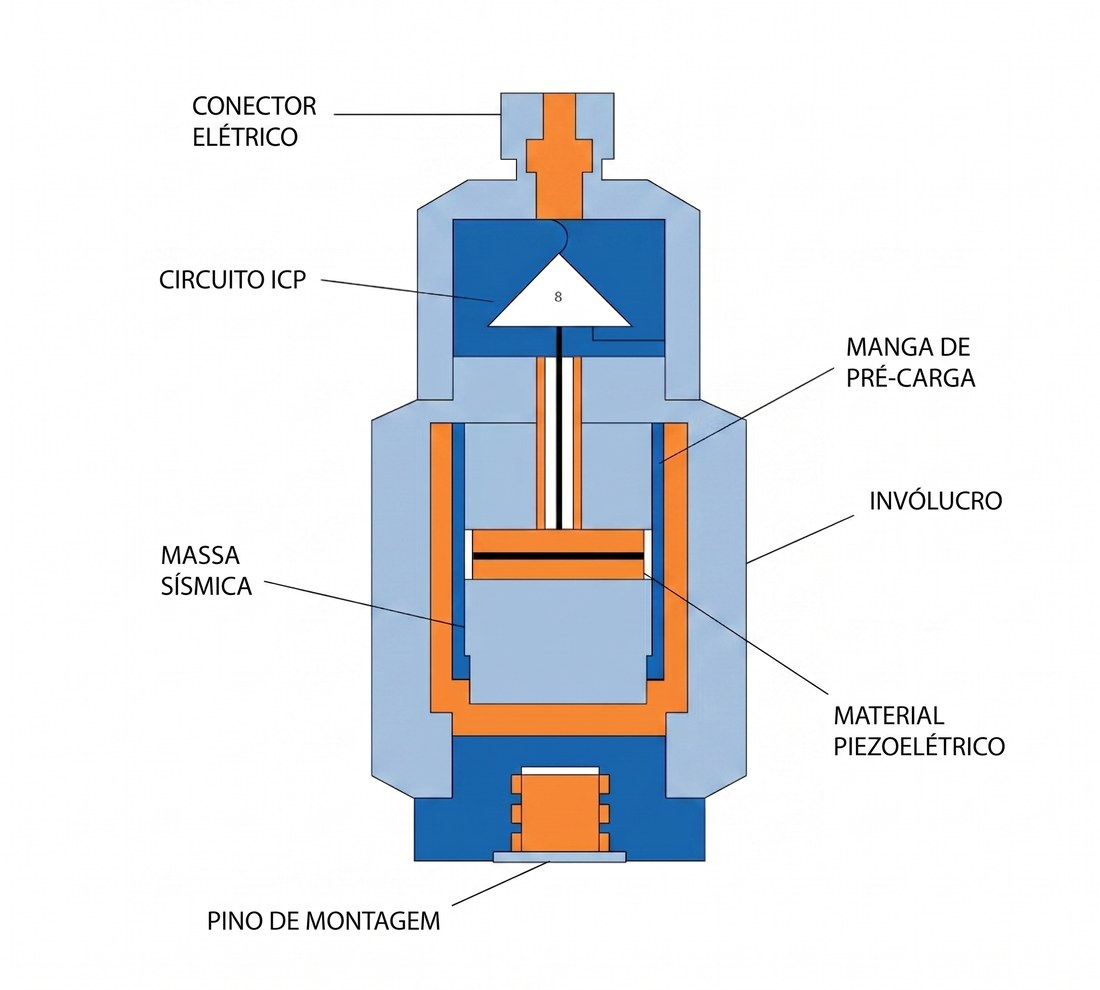
\includegraphics[width=\columnwidth]{Images/acelerometro_dewesoft traduzido.png}
    \caption{Acelerômetro de compressão piezoelétrico da Dewesoft. Fonte: \cite{aceletrometroDewesoft2025}.}
    \label{fig:acelerometro_dewesoft}
\end{figure}

Contudo, uma vez que é necessário fazer a montagem física dos sensores nas peças, limitações físicas e de acesso podem restringir ou impedir sua utilização em certos casos. Alguns exemplos de aplicações críticas incluem:

\begin{itemize}
    \item Monitoramento de vibrações em pás de rotores.
    \item Medição de vibrações em componentes muito leves ou frágeis.
    \item Componentes que trabalham em altas temperaturas.
\end{itemize}

Para contornar as limitações de instrumentação física, técnicas de vibrometria óptica têm sido cada vez mais utilizadas para a medição sem contato \cite{Phase2022}. Essas técnicas permitem a obtenção de informações sobre o comportamento dinâmico de estruturas sem o acréscimo indesejado de massa (\textit{mass loading}), o que é particularmente vantajoso em sistemas sensíveis. Uma das técnicas ópticas consagradas é a vibrometria por Laser Doppler (LDV) apresentada na Figura \ref{fig:ldv}. No entanto, apesar de sua alta fidelidade e precisão \cite{LDVpolytec2006}, sistemas LDV industriais apresentam custos de aquisição e manutenção bastante elevados, além de exigirem \textit{setups} experimentais complexos e realizarem medições limitadas a pontos específicos (espacialmente discretas). Isso enfatiza a necessidade de alternativas que mantenham a natureza não intrusiva, mas com maior viabilidade econômica e capacidade de monitoramento global.

\begin{figure}[htbp]
    \centering
    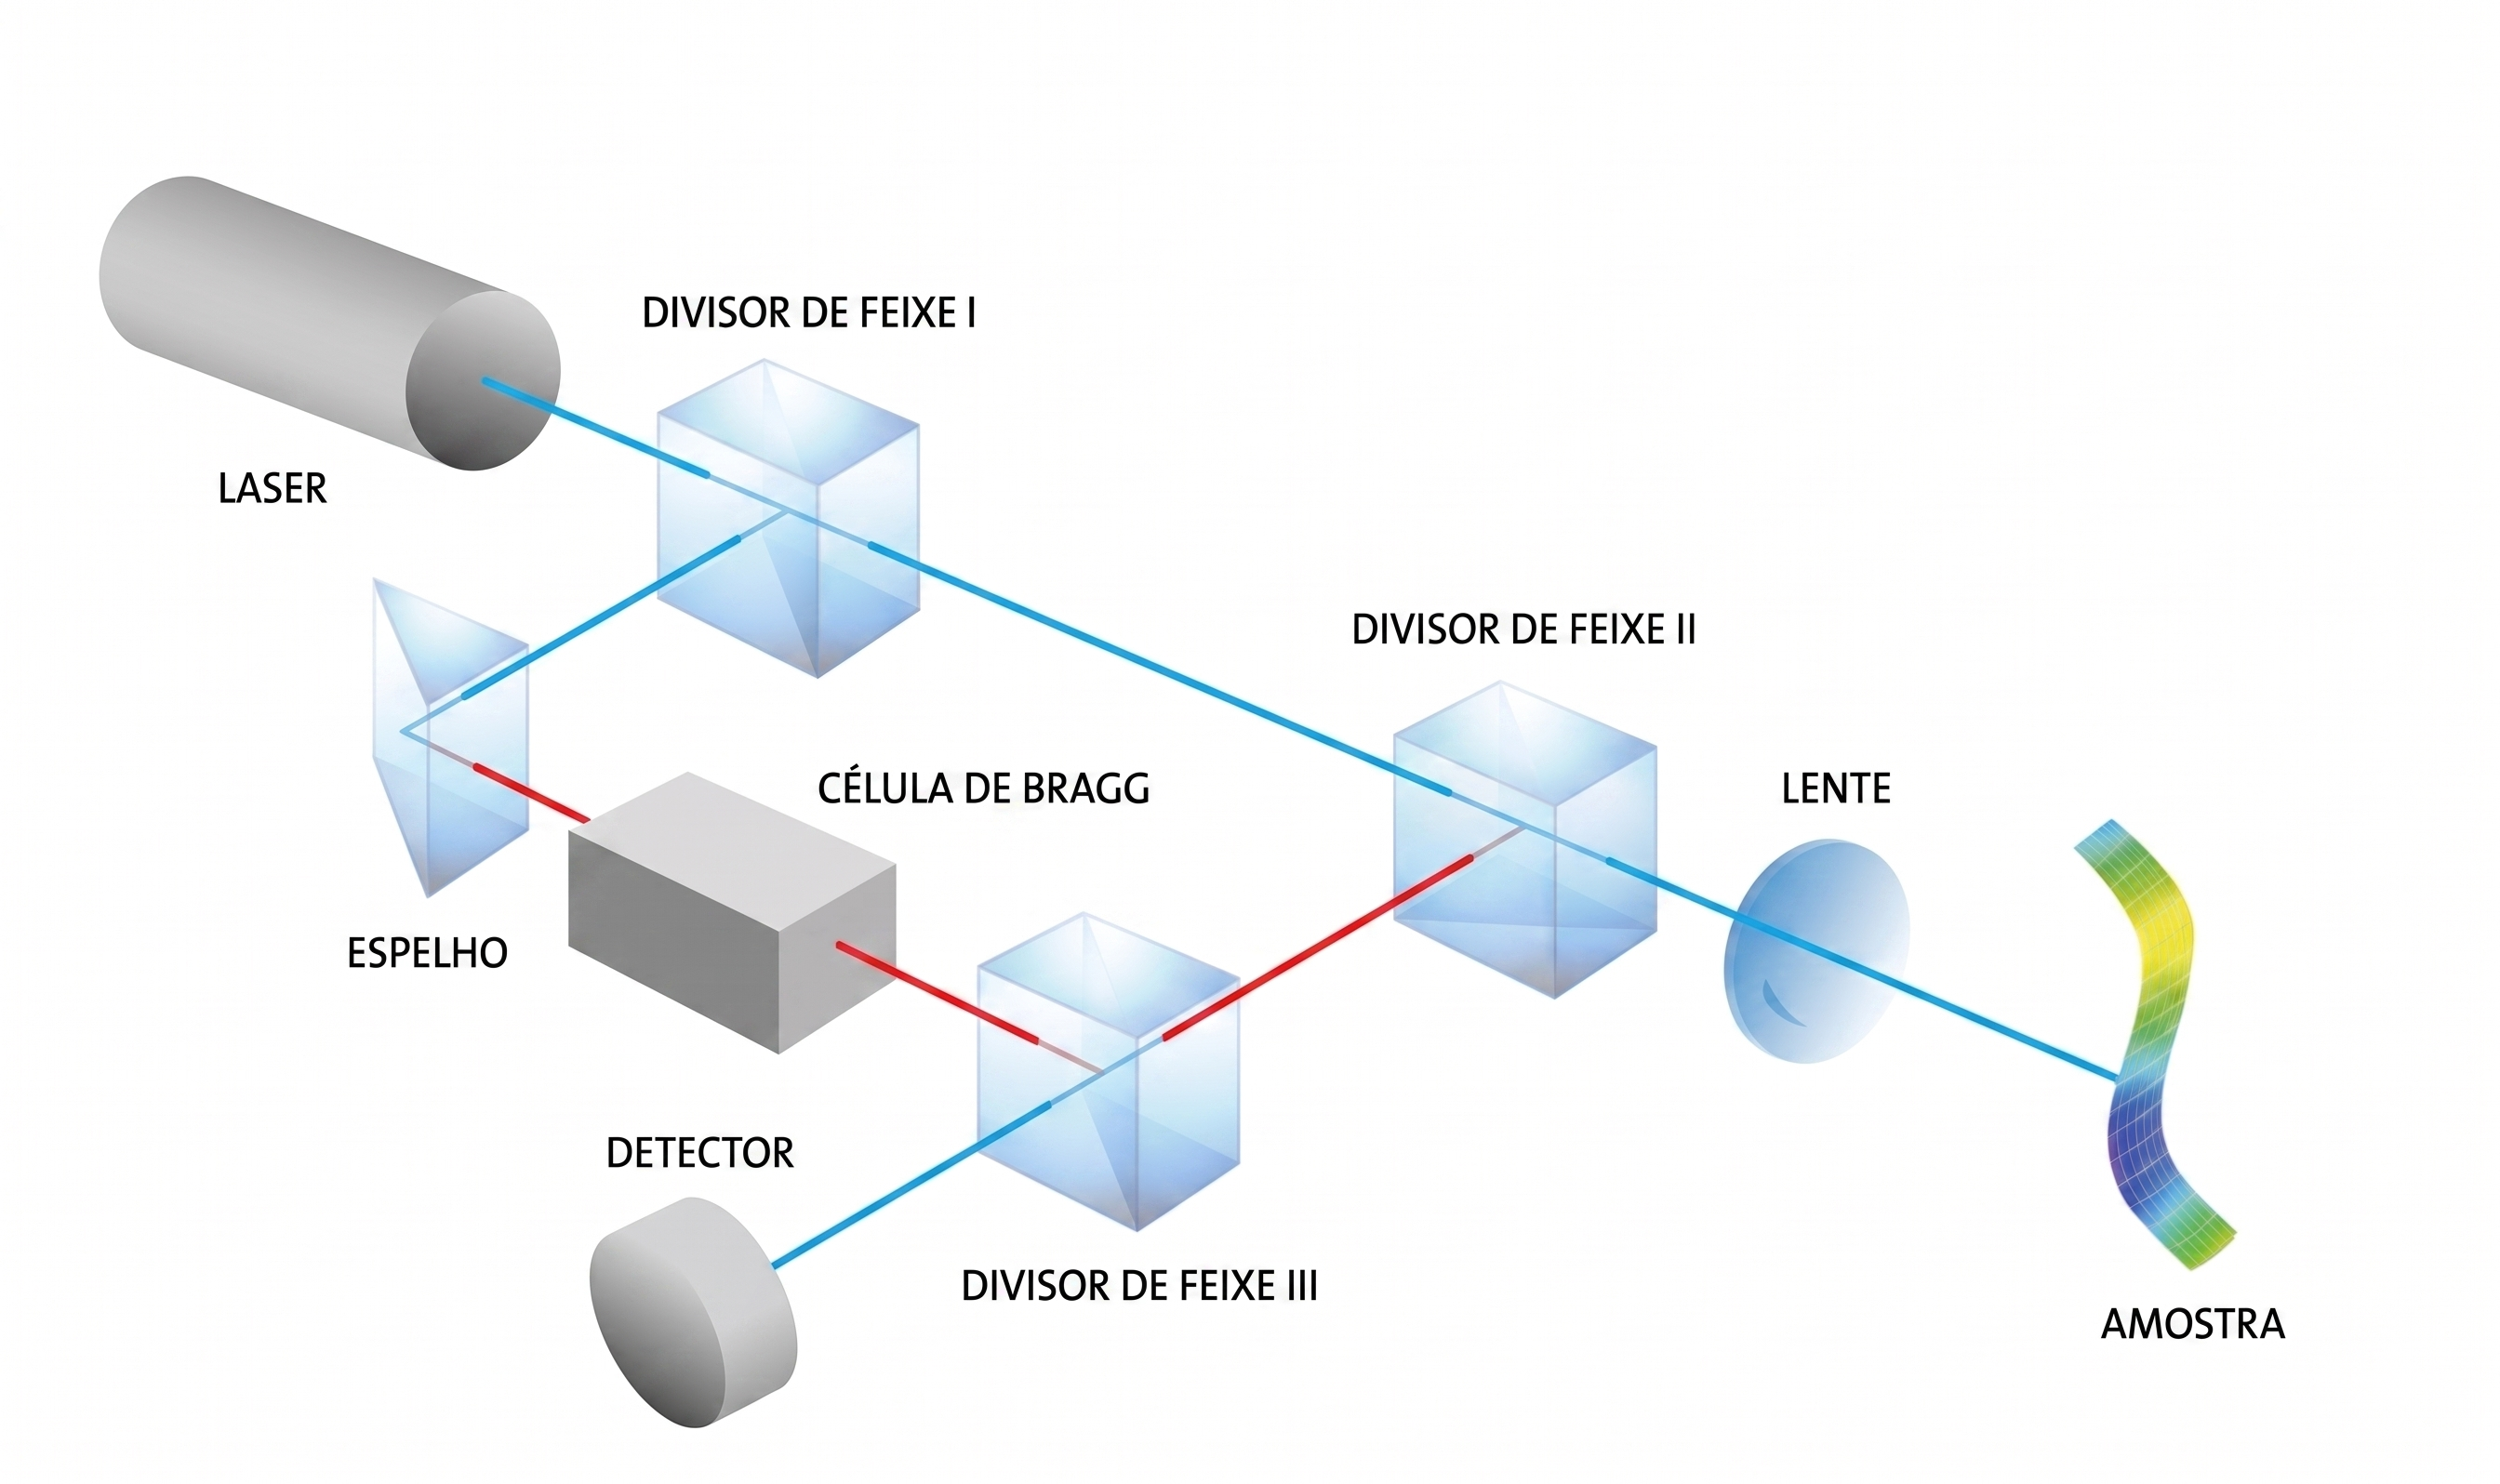
\includegraphics[width=\columnwidth]{Images/LDV traduzido.png}
    \caption{Vibrometria por Laser Doppler. Fonte: \cite{LDVpolytec2006}.}
    \label{fig:ldv}
\end{figure}

Uma alternativa promissora é a vibrometria por imagem, que utiliza câmeras de vídeo convencionais para capturar o movimento vibracional de uma estrutura. Através de técnicas avançadas de processamento digital de imagens (\textit{phase-based} e amplificação de movimento), é possível extrair informações sobre a amplitude e frequência das vibrações, permitindo uma análise detalhada do comportamento dinâmico da estrutura \cite{robotcamera2025}. Essa abordagem tem o potencial de ser uma solução de baixo custo e fácil implementação para monitoramento de vibrações em tempo real, especialmente em ambientes onde a instalação de sensores físicos é inviável.

O maior desafio dessa abordagem se encontra na necessidade de estabilização de vídeo e na capacidade do equipamento de captura de vídeo em lidar com frequências muito altas e de amplitudes muito baixas, o que pode limitar a precisão e a aplicabilidade em certos cenários de teste. No entanto, avanços recentes em algoritmos de processamento de imagens e melhorias na qualidade das câmeras de vídeo estão continuamente expandindo as possibilidades dessa técnica para aplicações industriais e de pesquisa \cite{Phase2022}. Um modelo de como pode ser montado um sistema de vibrometria por câmera baseada em imagem é apresentado na Figura \ref{fig:camerabased_vibrometry}.

\begin{figure}[htbp]
    \centering
    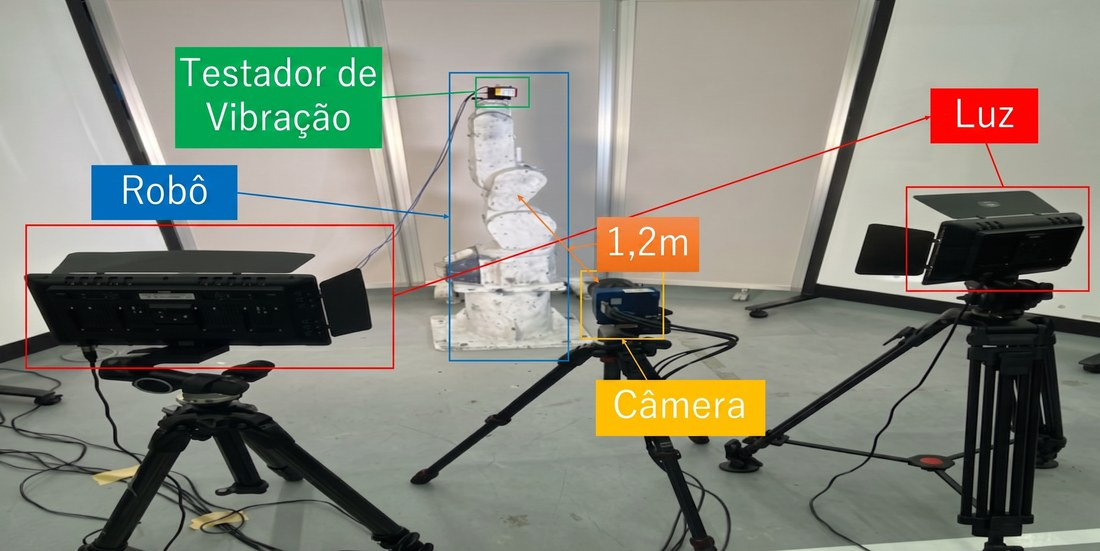
\includegraphics[width=\columnwidth]{Images/camerabased vibrometry traduzido.png}
    \caption{Vibrometria por câmera baseada em imagem. Fonte: \cite{robotcamera2025}.}
    \label{fig:camerabased_vibrometry}
\end{figure}

O grande diferencial desta técnica em relação aos métodos tradicionais de contato (e até mesmo ao LDV pontual) é a capacidade de obter um histórico visual contínuo da propagação de falhas mecânicas. Isso é particularmente valioso para a compreensão espacial dos modos de falha ao longo de todo o componente em teste, otimizando a segurança operacional e a análise forense.

\subsection{Problema}
Apesar da ampla utilização e eficácia dos acelerômetros em medições vibracionais, os sistemas tradicionais de testes em bancada baseiam-se, em geral, em medições pontuais e discretas, limitadas ao monitoramento de regiões específicas da estrutura. Essa abordagem pode não capturar de forma completa o comportamento dinâmico global do sistema, além de, em alguns casos, exigir ensaios destrutivos que acarretam prejuízos devido à perda ou danificação do equipamento testado.

Nesse contexto, a aplicação da vibrometria óptica por câmeras e visão computacional surge como uma boa alternativa, não para substituir os métodos tradicionais, mas para complementá-los, por possibilitar medições sem contato e com maior resolução espacial. Contudo, sua implementação em testes dinâmicos de bancada ainda apresenta desafios relevantes, tais como a necessidade de condições controladas de iluminação, a elevada sensibilidade a ruídos ambientais e a complexidade computacional envolvida na aquisição, processamento e interpretação dos dados obtidos \cite{Phase2022}.

\subsection{Objetivos}

O objetivo geral deste trabalho é explorar e validar a aplicação de metodologias não intrusivas de vibrometria óptica para medição de vibrações em testes dinâmicos de bancada, buscando superar os desafios de instrumentação.

\noindent\textit{Objetivos Específicos:}
\begin{itemize}
    \item Desenvolver e implementar rotinas de processamento digital de imagens em ambiente Python, baseadas em filtragem por convolução com filtros de Gabor para estimativa de movimento baseada em fase, aplicadas ao monitoramento da integridade estrutural (\textit{Structural Health Monitoring} -- SHM);
    \item Propor e validar uma metodologia não intrusiva de baixo custo, baseada no uso de câmeras de vídeo convencionais, para a medição de vibrações;
    \item Comparar o desempenho da abordagem óptica com os métodos tradicionais de medição por contato, analisando precisão, confiabilidade e limitações.
\end{itemize}

\subsection{Justificativa}
O desenvolvimento e a validação de um sistema de medição sem contato e de baixo custo justificam-se pela necessidade contínua de segurança operacional (\textit{safety margin}) em ensaios de durabilidade. Ao contornar as limitações físicas dos sensores tradicionais, a abordagem óptica viabiliza a criação de um histórico visual e contínuo da iniciação e propagação de falhas mecânicas. Dessa forma, demonstra-se não apenas as vantagens dessa abordagem em comparação aos métodos tradicionais, mas também garante-se uma alta viabilidade econômica e mais ferramentas de análise forense para compreensão de modos de falha ao longo de todo o componente em teste.

\section{Fundamentação Teórica}

\subsection{Conceitos Fundamentais de Dinâmica e Vibrações Mecânicas}

Antes de discutir transdutores e técnicas de medição, é necessário caracterizar o fenômeno a ser medido. Vibração mecânica é, em essência, a oscilação de um sistema em torno de uma posição de equilíbrio, sustentada pela troca contínua entre energia potencial (armazenada em elementos elásticos) e energia cinética (associada ao movimento de massa) \cite{Downey2026, Rao2010}. Presente em praticamente todo sistema mecânico real, o fenômeno pode ser desejável (peneiras vibratórias, lixadeiras orbitais) ou destrutivo (ressonâncias em estruturas aeronáuticas e civis), e seu correto modelamento é etapa fundamental no projeto e na manutenção de máquinas e estruturas.

\subsubsection{Sistema massa-mola-amortecedor de 1 GDL}

O modelo mais simples capaz de descrever um sistema vibratório é o de um grau de liberdade (1~GDL), composto por uma massa concentrada $m$, uma mola linear de rigidez $k$ e um amortecedor viscoso de coeficiente $c$. Aplicando-se a segunda lei de Newton, obtém-se a equação de movimento (EOM) na forma padrão \cite{Downey2026}:
\begin{equation}
    m\ddot{x}(t) + c\dot{x}(t) + k\,x(t) = F(t),
    \label{eq:eom_1gdl}
\end{equation}
em que $F(t)$ é uma eventual força externa aplicada. No caso de vibração livre, $F(t) = 0$, e a Equação \ref{eq:eom_1gdl} se torna uma equação diferencial linear homogênea de segunda ordem, cuja resolução conduz aos parâmetros fundamentais do sistema: a frequência natural não amortecida $\omega_n = \sqrt{k/m}$ e a razão de amortecimento adimensional $\zeta = c/(2m\omega_n)$.

Essa razão $\zeta$ classifica o sistema em três regimes de resposta livre (Tabela \ref{tab:casos_amortecimento}): subamortecido ($0 < \zeta < 1$), criticamente amortecido ($\zeta = 1$) e superamortecido ($\zeta > 1$) \cite{Downey2026}. A grande maioria dos sistemas mecânicos reais opera no regime subamortecido, em que a resposta livre toma a forma de uma oscilação decrescente exponencialmente:
\begin{equation}
    x(t) = A\,e^{-\zeta \omega_n t}\sin(\omega_d t + \phi),
    \label{eq:resposta_subamortecida}
\end{equation}
com $\omega_d = \omega_n\sqrt{1 - \zeta^2}$ a frequência natural amortecida. Tanto $\omega_d$ quanto $\zeta$ podem ser extraídos diretamente de um sinal experimental de resposta livre, por meio de análise espectral e do decremento logarítmico, respectivamente \cite{Downey2026, Rao2010}.

\begin{table}[htbp]
    \centering
    \caption{Regimes de resposta livre em função da razão de amortecimento $\zeta$.}
    \label{tab:casos_amortecimento}
    \small
    \begin{tabularx}{\columnwidth}{l c X}
        \toprule
        \textbf{Regime} & \textbf{$\zeta$} & \textbf{Natureza da resposta} \\
        \midrule
        Não amortecido          & $\zeta = 0$     & Oscilação harmônica permanente. \\
        Subamortecido           & $0 < \zeta < 1$ & Oscilação com decaimento exponencial. \\
        Criticamente amortecido & $\zeta = 1$     & Retorno ao equilíbrio sem oscilação. \\
        Superamortecido         & $\zeta > 1$     & Retorno lento ao equilíbrio. \\
        \bottomrule
    \end{tabularx}
\end{table}

A Figura \ref{fig:regimes_amortecimento} ilustra os diferentes regimes de resposta livre para um sistema de 1~GDL, evidenciando a influência da razão de amortecimento na forma do sinal temporal.

\begin{figure}[htbp]
    \centering
    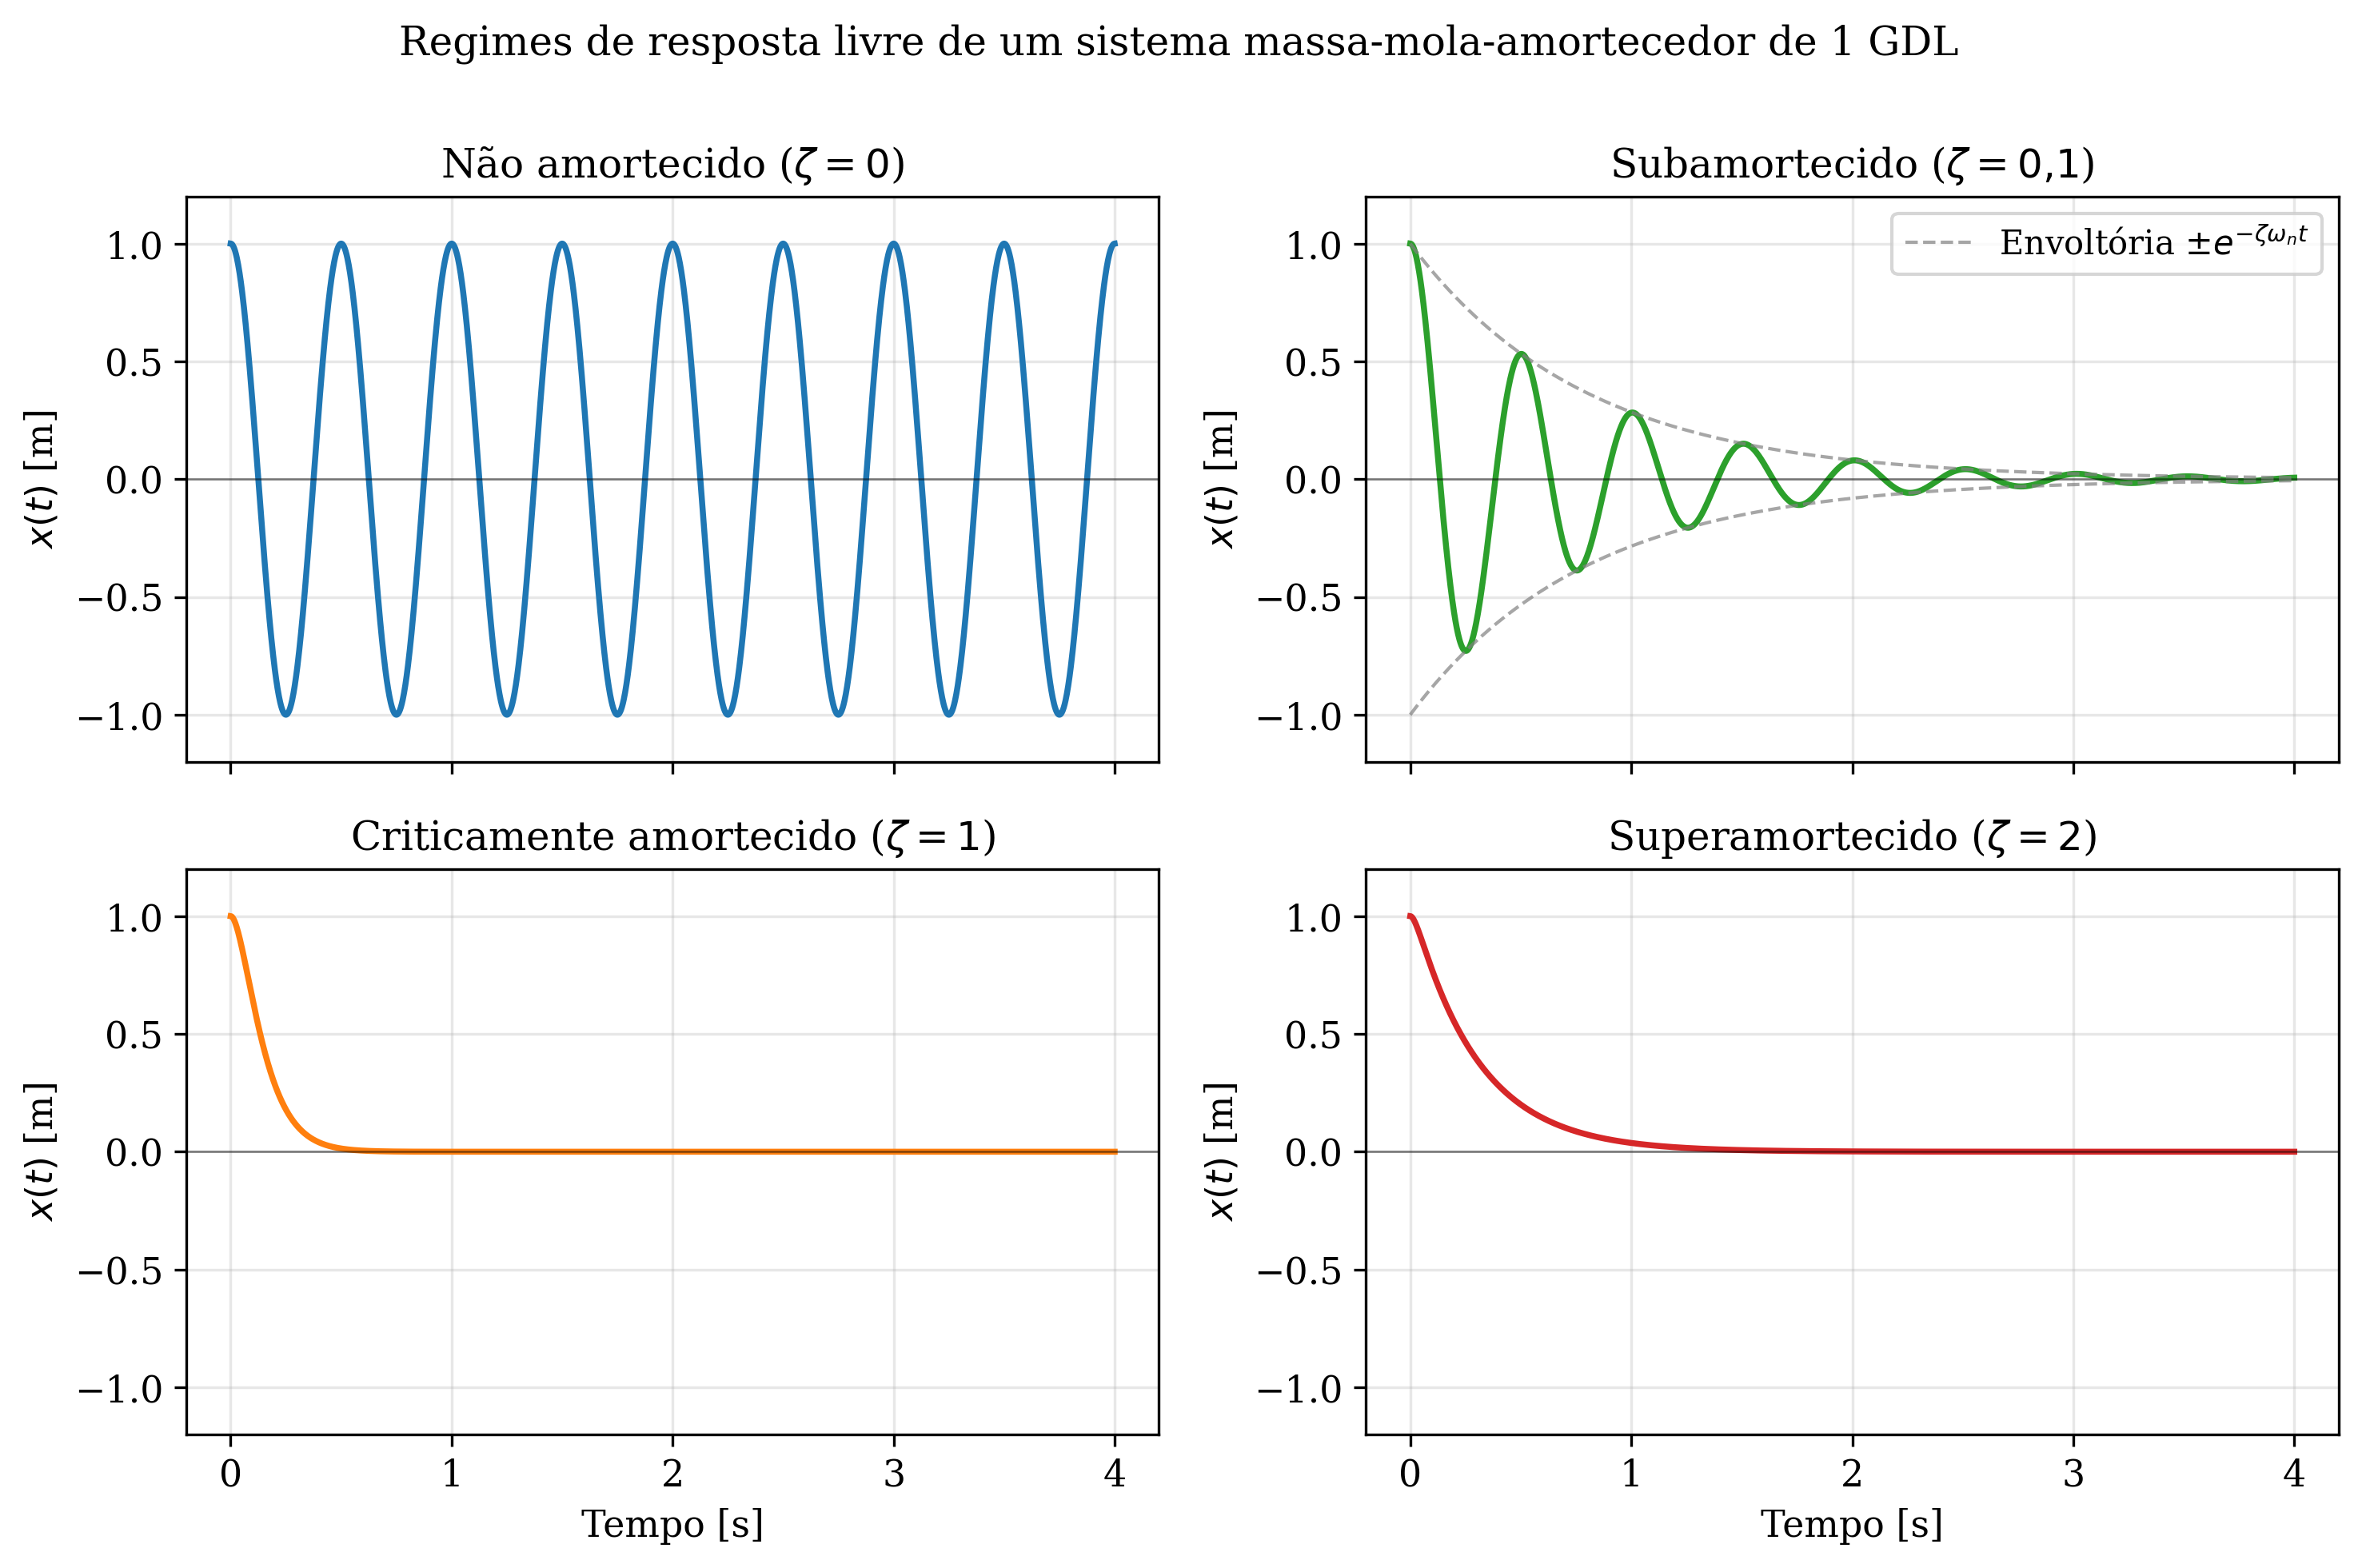
\includegraphics[width=\columnwidth]{Images/fig_regimes_amortecimento.png}
    \caption{Respostas de regime de amortecimento. Fonte: O autor.}
    \label{fig:regimes_amortecimento}
\end{figure}

\subsubsection{Vibração forçada e ressonância}

Quando o sistema é submetido a uma excitação harmônica do tipo $F(t) = F_0\cos(\omega t)$, a solução da EOM é composta por uma parcela transitória, que se extingue após alguns ciclos, e uma parcela permanente que governa o comportamento de longo prazo. A amplitude da resposta permanente é dada por \cite{Downey2026}:
\begin{equation}
    X = \frac{F_0/k}{\sqrt{(1 - r^2)^2 + (2\zeta r)^2}},
    \label{eq:amplitude_forcada}
\end{equation}
em que $r = \omega/\omega_n$ é a razão de frequências adimensional. A relação entre a amplitude normalizada e $r$ define a Função de Resposta em Frequência (FRF) do sistema, ferramenta central da análise vibracional experimental.

A condição de ressonância ocorre quando $\omega$ se aproxima de $\omega_n$ ($r \approx 1$). No caso não amortecido, a Equação \ref{eq:amplitude_forcada} diverge, e mesmo em sistemas com amortecimento real a amplitude pode atingir valores várias ordens de grandeza maiores do que aqueles observados fora da banda de ressonância. Esse fenômeno é a causa raiz de inúmeras falhas estruturais documentadas e justifica a necessidade de mapear as frequências naturais antes de colocar um componente em operação \cite{Downey2026, Rao2010}. Esse comportamento pode ser evidenciado na Figura \ref{fig:ressonancia}, onde a FRF apresenta um pico acentuado na frequência de ressonância, cuja amplitude é inversamente proporcional à razão de amortecimento $\zeta$.

\begin{figure}[htbp]
    \centering
    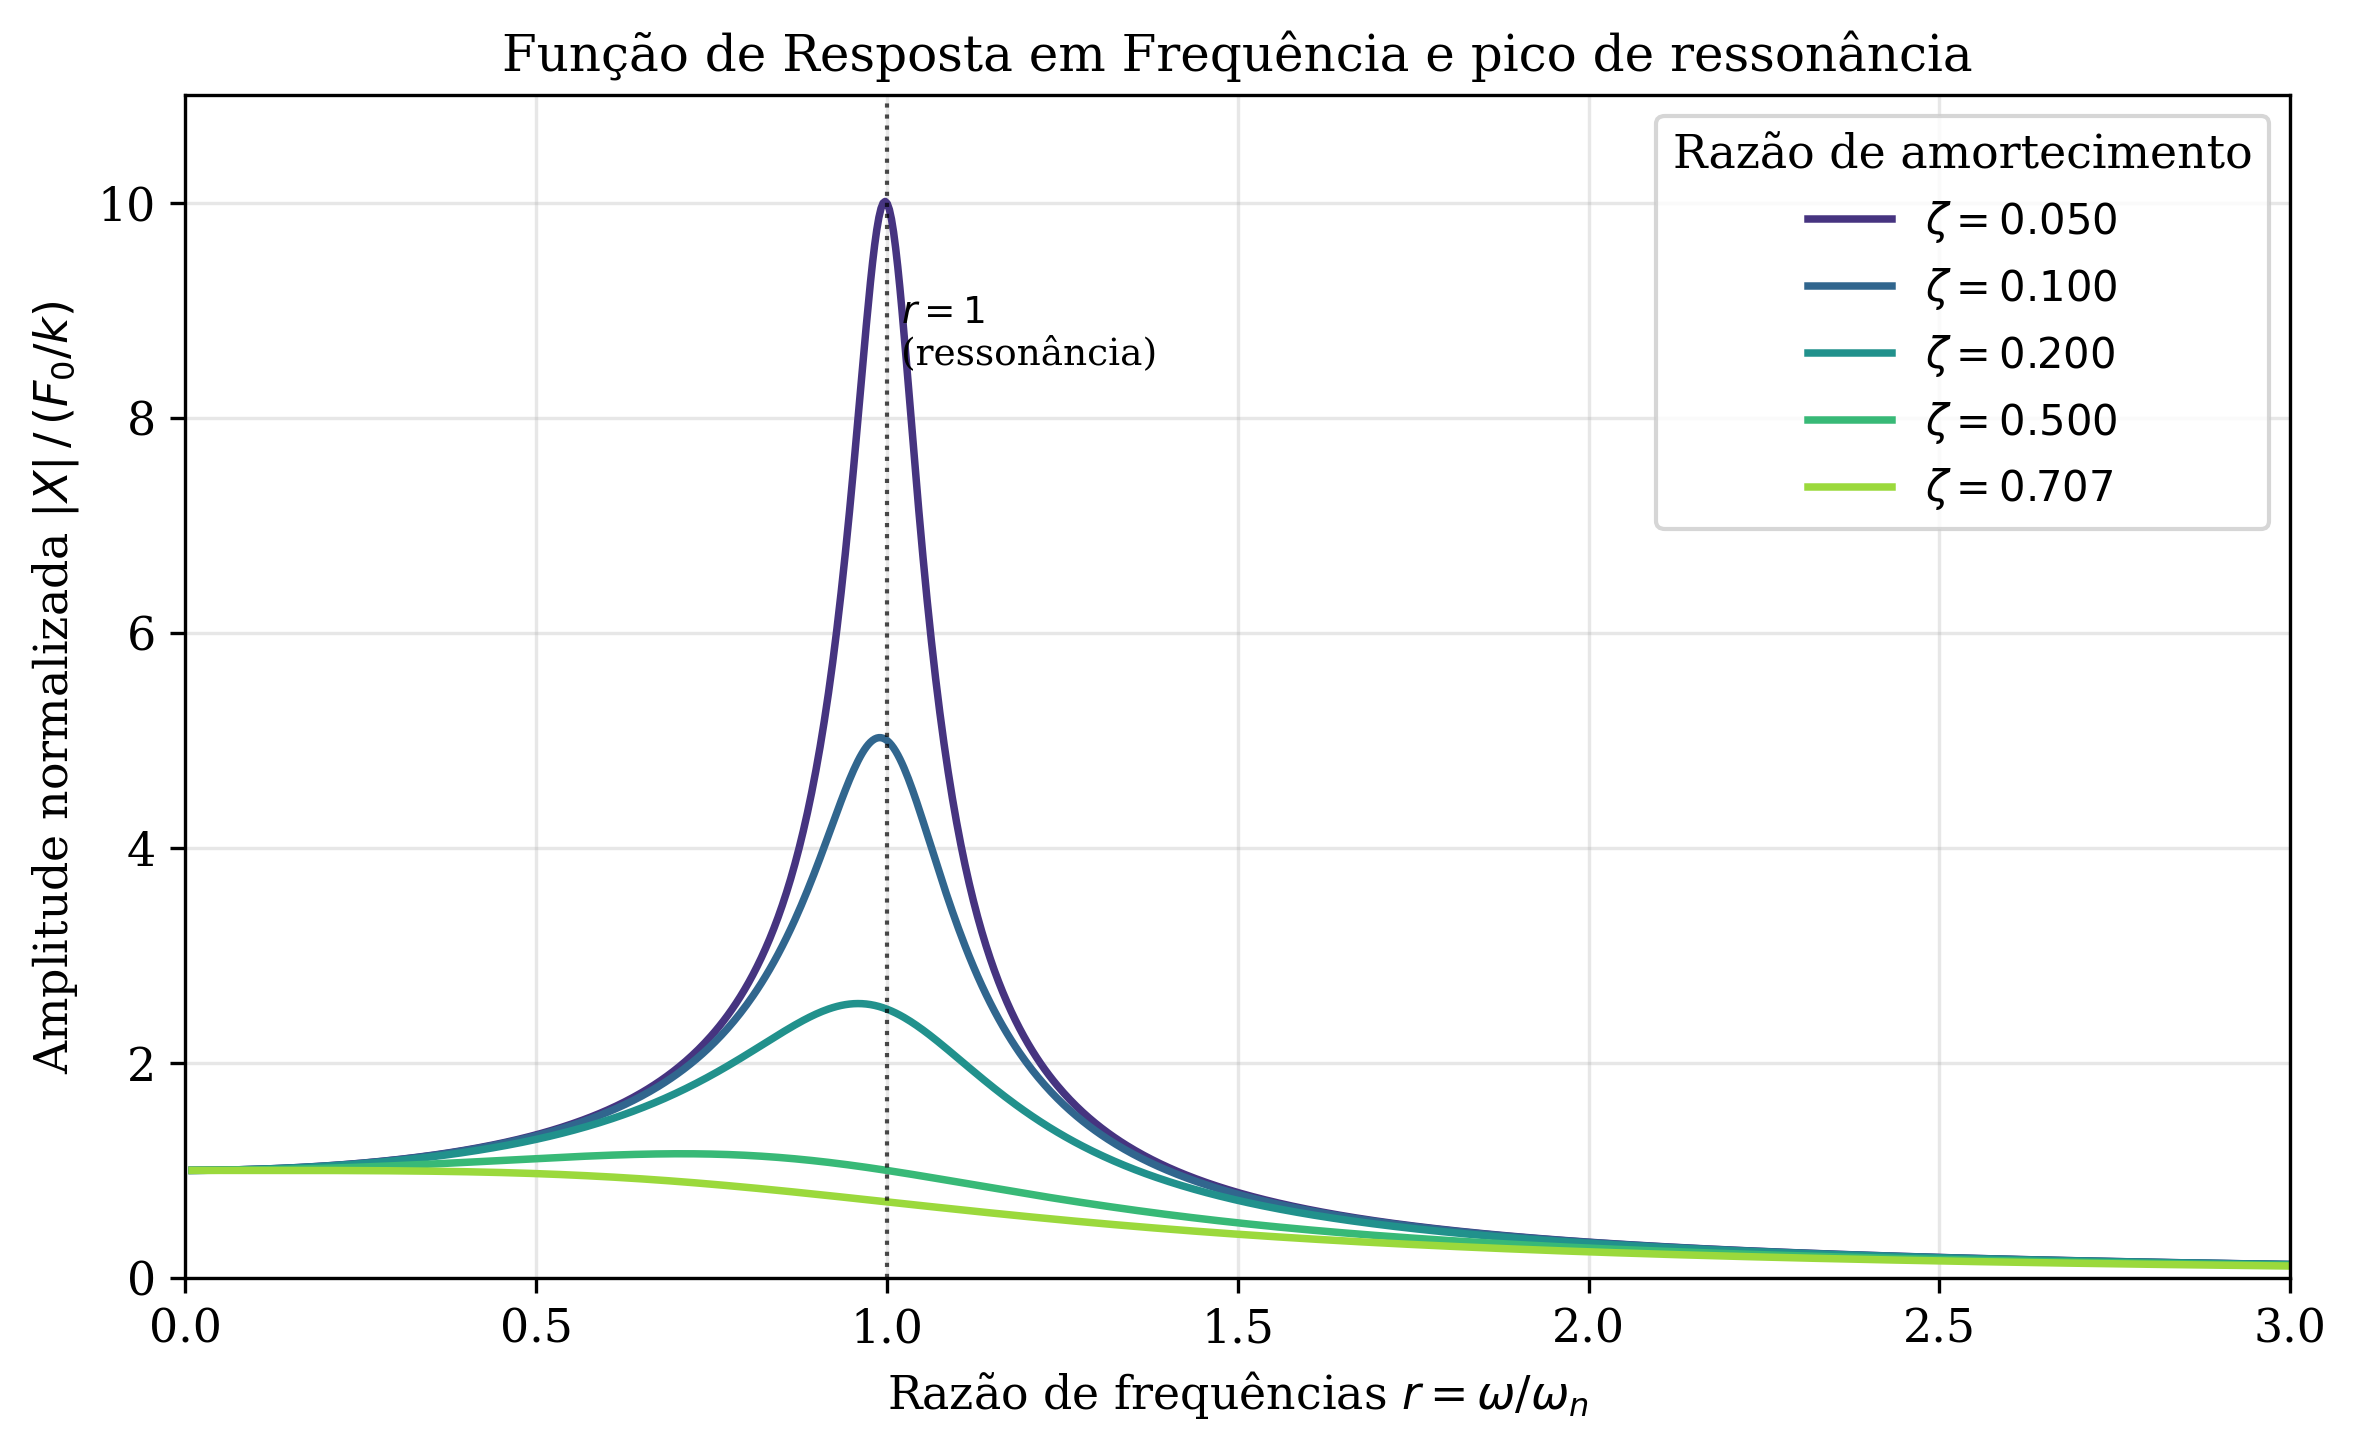
\includegraphics[width=\columnwidth]{Images/fig_ressonancia.png}
    \caption{Função de Resposta em Frequência e pico de ressonância. Fonte: O autor.}
    \label{fig:ressonancia}
\end{figure}

No contexto deste trabalho, o caso da excitação de base é particularmente relevante, pois corresponde ao cenário dos ensaios dinâmicos de bancada com excitadores eletromagnéticos (\textit{shakers}) e atuadores hidráulicos (\textit{rigs}), nos quais o componente sob análise é montado sobre uma plataforma com aceleração controlada \cite{Downey2026}.

\subsubsection{Sistemas de múltiplos graus de liberdade e análise modal}

Estruturas reais raramente são adequadamente representadas por um único grau de liberdade. Quando duas ou mais coordenadas independentes são necessárias para descrever a configuração do sistema, fala-se em sistemas de múltiplos graus de liberdade (MGDL). A EOM, agora vetorial, é convenientemente expressa em forma matricial \cite{Downey2026, Rao2010}:
\begin{equation}
    \mathbf{M}\,\ddot{\vec{x}}(t) + \mathbf{C}\,\dot{\vec{x}}(t) + \mathbf{K}\,\vec{x}(t) = \vec{F}(t),
    \label{eq:eom_mdof}
\end{equation}
em que $\mathbf{M}$, $\mathbf{C}$ e $\mathbf{K}$ são as matrizes de massa, amortecimento e rigidez do sistema. Para o caso não amortecido em vibração livre, a substituição de uma solução harmônica resulta em um problema de autovalor cuja solução fornece pares de frequências naturais $\omega_i$ e modos de vibrar $\vec{u}_i$ (\textit{mode shapes}) \cite{Downey2026}.

A interpretação física é central para o presente trabalho: um modo de vibrar não representa o deslocamento absoluto do sistema, mas sim o \textit{padrão espacial} de oscilação que a estrutura assume naturalmente quando excitada na frequência correspondente. A obtenção experimental desses pares constitui a análise modal experimental (\textit{Experimental Modal Analysis}), área consolidada da dinâmica estrutural \cite{Ewins2000}. É justamente nesse ponto que se manifesta a maior limitação dos métodos por contato: como os acelerômetros fornecem informação \textit{pontual}, a reconstrução de um modo de vibrar com boa resolução espacial exige um grande número de sensores ou múltiplas montagens sequenciais. A vibrometria por imagem, em contraposição, oferece naturalmente a capacidade de campo completo (\textit{full-field}), motivando sua investigação como complemento aos métodos consagrados \cite{robotcamera2025}.

\subsubsection{Structural Health Monitoring (SHM) e assinatura vibracional}

O \textit{Structural Health Monitoring} (SHM) consiste no processo contínuo ou periódico de aquisição, processamento e interpretação de dados oriundos de uma estrutura, com o objetivo de detectar, localizar e caracterizar danos antes que estes evoluam para falha catastrófica \cite{Doebling1998}. No contexto vibracional, o SHM se apoia em uma premissa direta: como os parâmetros modais (frequências naturais, modos de vibrar e razões de amortecimento) são funções das propriedades físicas do sistema (massa, rigidez e amortecimento), alterações nessas propriedades introduzidas por trincas, perda de seção resistente, afrouxamento de fixações ou desgaste resultam em mudanças mensuráveis nas propriedades modais \cite{Doebling1998}.

Considerando o sistema de 1~GDL, uma perda localizada de rigidez $\Delta k < 0$ desloca a frequência natural para $\omega_n' = \sqrt{(k + \Delta k)/m} < \omega_n$, ou seja, danos estruturais tendem a reduzir as frequências naturais observadas, ao passo que folgas e trincas tendem a aumentar a razão de amortecimento $\zeta$, alargando os picos da FRF. Esses dois efeitos constituem a base da chamada assinatura vibracional do componente. Em sistemas de MGDL, indicadores adicionais ficam disponíveis, como variações nas componentes dos modos de vibrar (especialmente em suas curvaturas) e alterações na FRF em bandas de frequência específicas \cite{Doebling1998}, todos mais sensíveis a danos localizados do que o simples deslocamento de frequência natural. Essa perda de rigidez pode ser visualizada na Figura \ref{fig:perda_rigidez}.

\begin{figure}[htbp]
    \centering
    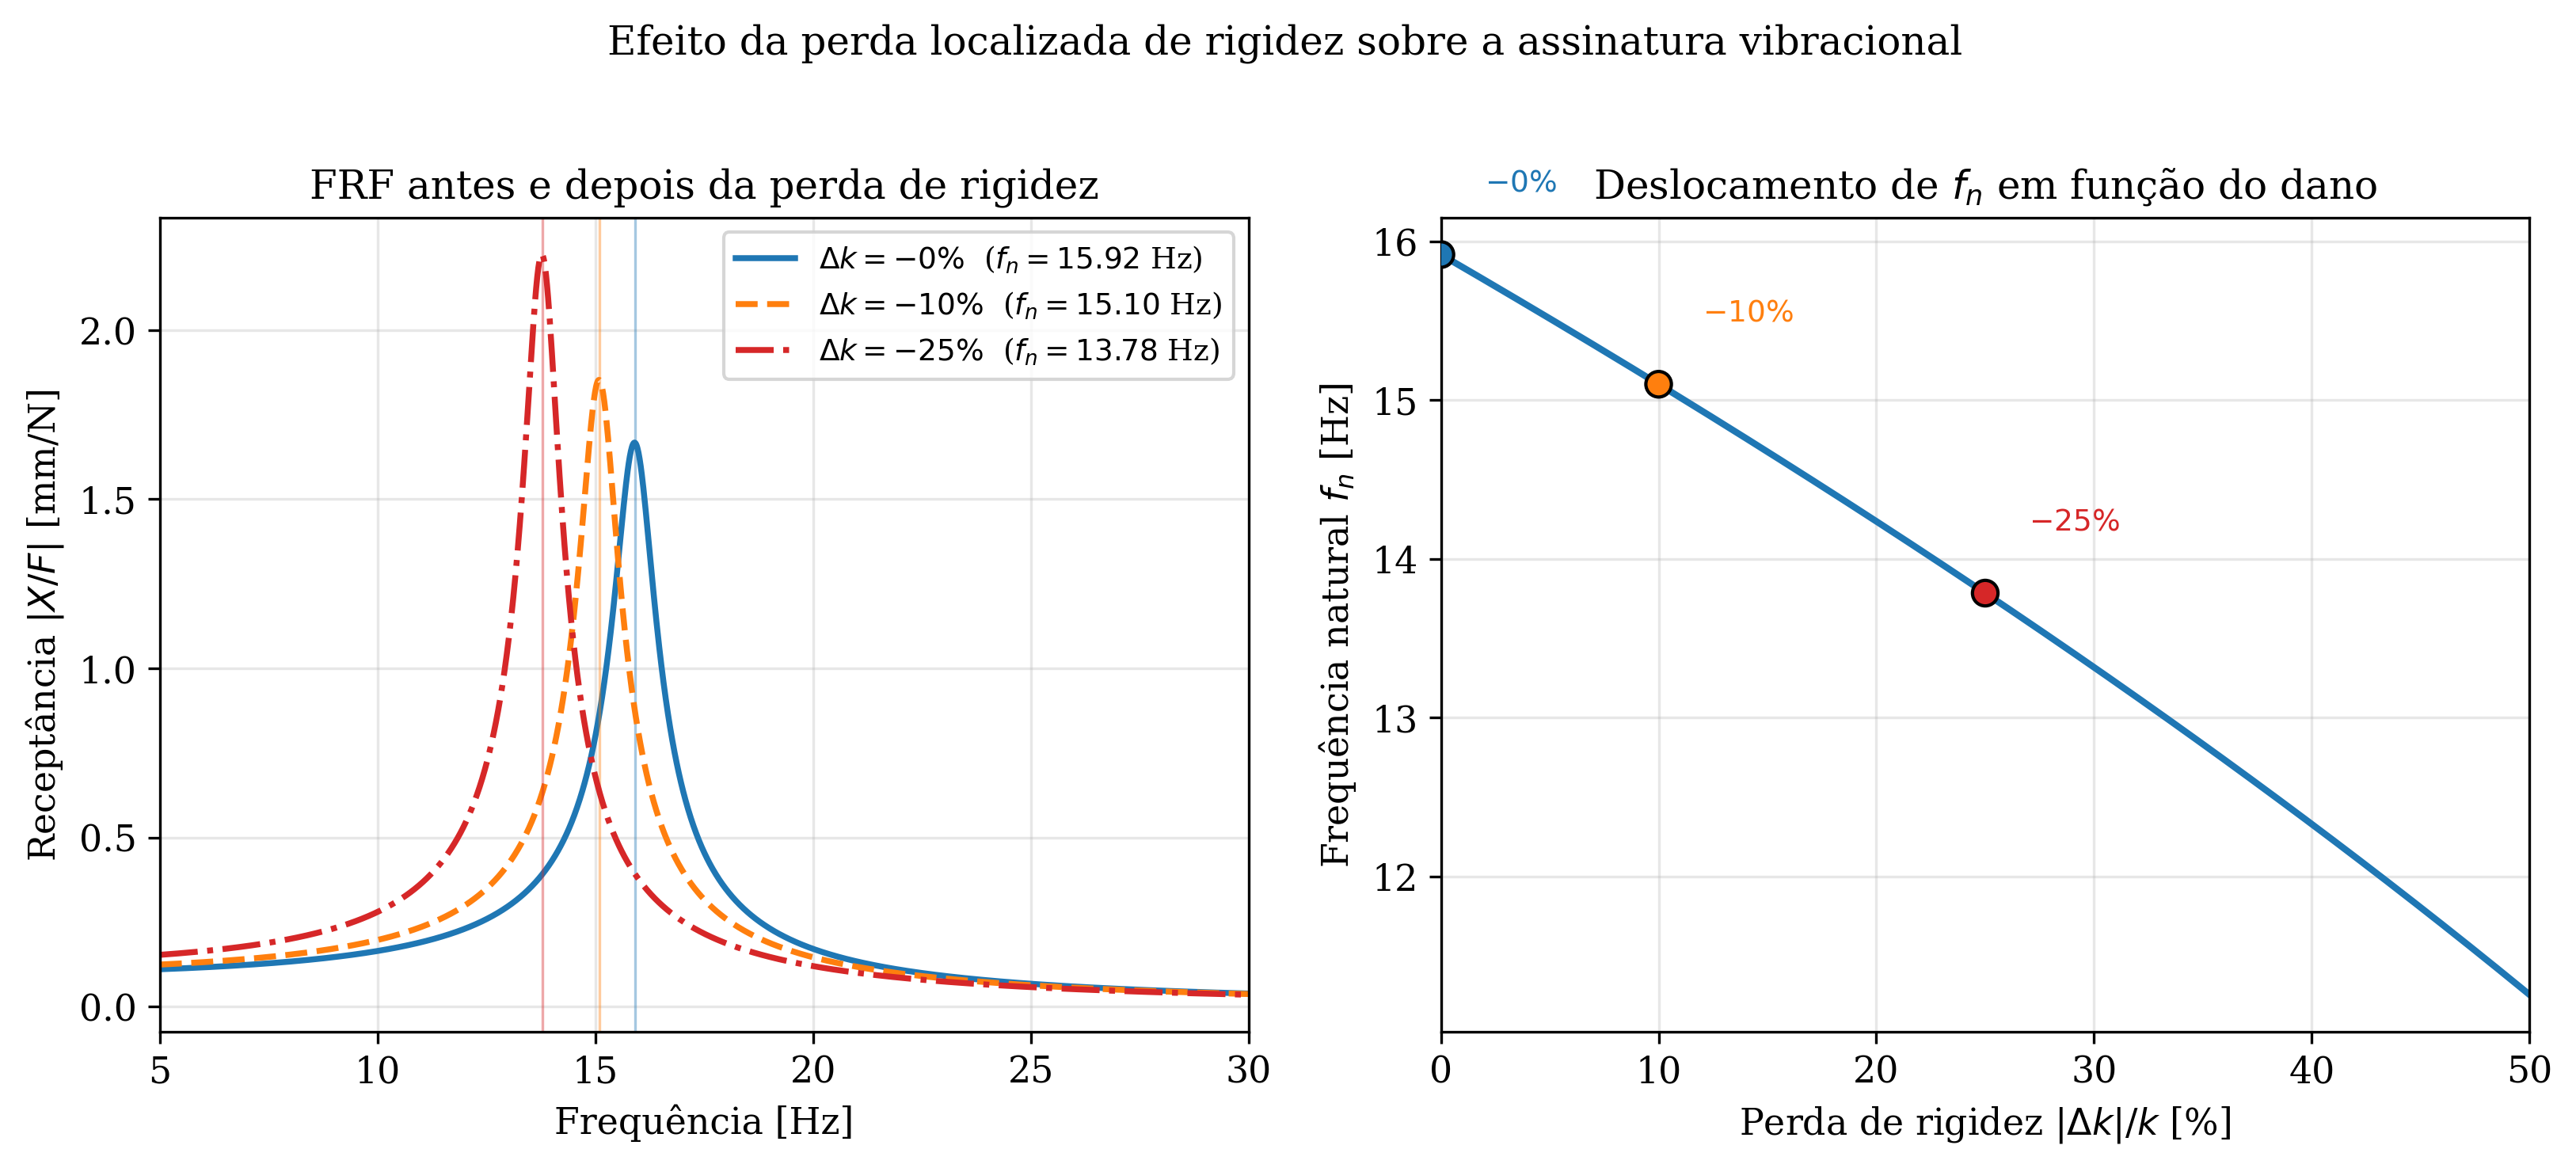
\includegraphics[width=\columnwidth]{Images/fig_perda_rigidez.png}
    \caption{Resposta de sistema submetido a perda de rigidez. Fonte: O autor.}
    \label{fig:perda_rigidez}
\end{figure}

Como aplicação a jusante dessa cadeia, os históricos temporais de deslocamento obtidos por qualquer método de medição (incluindo a vibrometria óptica investigada neste trabalho) podem alimentar análises clássicas de fadiga, em que ciclos de carregamento são contabilizados pelo método de \textit{rainflow counting} \cite{ASTM_E1049} e convertidos em dano acumulado por meio da regra linear de Palmgren-Miner \cite{Miner1945}. Essa ponte conecta a medição de vibrações a estimativas de vida útil, ampliando o escopo de aplicação da técnica em ensaios de durabilidade.

\subsection{Instrumentação Tradicional por Contato: Acelerômetros}

Os acelerômetros, já apresentados na contextualização, são transdutores inerciais que convertem aceleração mecânica em sinal elétrico. Internamente, todos compartilham um mesmo princípio físico: um sistema massa-mola-amortecedor em miniatura, no qual uma massa sísmica $m_s$ aplica uma força inercial sobre um elemento sensor à medida que a base do dispositivo é acelerada \cite{Downey2026}. Pela segunda lei de Newton, essa força é proporcional à aceleração da base, e a deformação resultante no elemento sensor é convertida em sinal elétrico mensurável. A faixa útil de operação do sensor é necessariamente bem abaixo de sua frequência natural interna, justamente para que a massa sísmica acompanhe fielmente o movimento da base.

\subsubsection{Tecnologias de transdução}

A natureza física do elemento sensor define a tecnologia de transdução e, consequentemente, as características e limitações do acelerômetro \cite{PiezoAccelerometer2023}:

\begin{itemize}
    \item Piezoelétricos: utilizam cristais (quartzo) ou cerâmicas polarizadas (PZT) que geram carga elétrica proporcional à força aplicada. Apresentam ampla faixa dinâmica, robustez e frequência de operação que pode chegar à ordem de dezenas de kHz, sendo o tipo predominante em aplicações industriais de média e alta frequência \cite{PiezoAccelerometer2023, aceletrometroDewesoft2025}. Por exigirem força dinâmica para gerar carga, não medem aceleração estática (DC).
    \item Piezorresistivos: empregam extensômetros em ponte de Wheatstone cuja resistência varia com a deformação. Medem componente DC e respondem bem a impactos e baixas frequências.
    \item Capacitivos (tipicamente MEMS): baseiam-se na variação de capacitância entre placas separadas pela massa sísmica. Permitem medição DC, têm baixo custo e dimensões reduzidas, mas com faixa dinâmica e frequência de operação mais limitadas \cite{Anna2026}.
    \item Ressonantes: a grandeza medida é o deslocamento da frequência de ressonância do elemento sensor causado pelo carregamento inercial. Oferecem altíssima precisão e são empregados em sistemas de navegação inercial.
\end{itemize}

\subsubsection{Efeito de mass loading e demais limitações práticas}

Apesar de consagrados, os acelerômetros impõem restrições importantes que motivam a busca por alternativas sem contato. A principal delas é o chamado efeito de \textit{mass loading}: ao ser fixado à peça em teste, o sensor adiciona massa ao sistema e desloca sua frequência natural local \cite{AgilentAN243-3, Ewins2000}. Para uma massa modal efetiva $m_{ef}$ no ponto de montagem, a frequência natural se modifica aproximadamente para
\begin{equation}
    \omega_n' = \omega_n \sqrt{\frac{m_{ef}}{m_{ef} + m_s}},
    \label{eq:mass_loading}
\end{equation}
em que $m_s$ é a massa total adicionada (sensor mais cabeamento e elemento de fixação) \cite{Serridge1987}. Para estruturas leves, por exemplo pás de rotores, painéis automotivos finos e componentes aeronáuticos, essa perturbação pode ser significativa e distorcer a medição da resposta natural \cite{AgilentAN243-3, robotcamera2025}, como exemplificado na Figura \ref{fig:mass_loading}.

\begin{figure}[htbp]
    \centering
    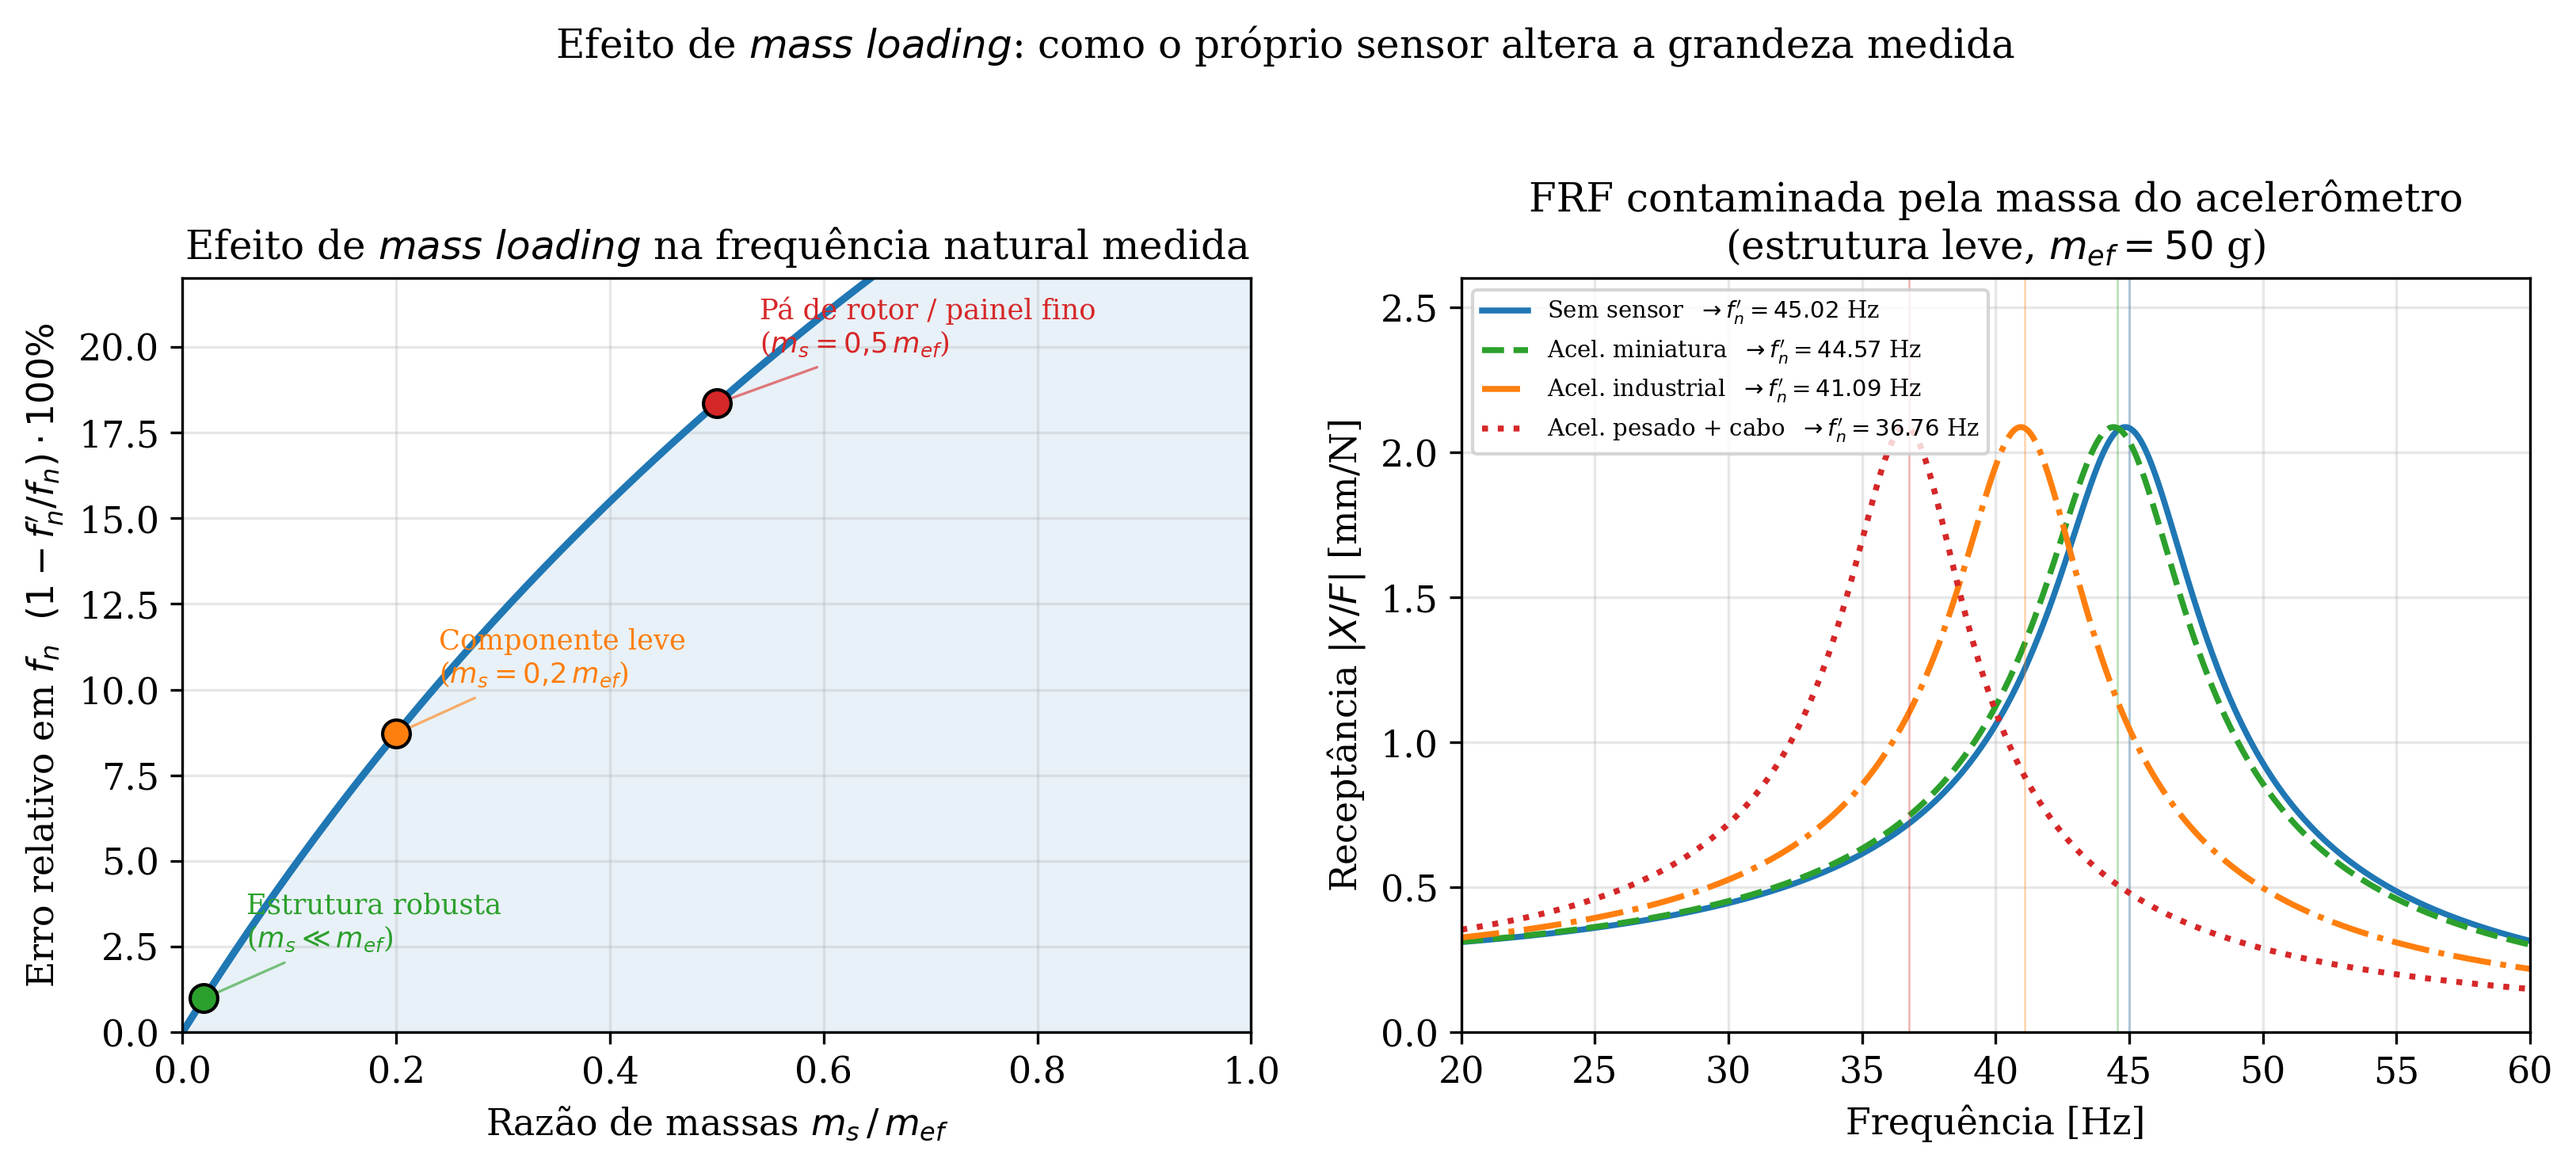
\includegraphics[width=\columnwidth]{Images/fig_mass_loading.png}
    \caption{Efeito de mass loading. Fonte: O autor.}
    \label{fig:mass_loading}
\end{figure}

Além do \textit{mass loading}, outras limitações práticas comprometem a aplicação dos acelerômetros em determinados cenários: o método de fixação (parafuso, cola, cera ou ímã) define uma frequência de corte adicional acima da qual o acoplamento mecânico deixa de ser rígido; o cabeamento introduz ruído triboelétrico e está sujeito a interferências eletromagnéticas; há restrições térmicas, em especial a chamada temperatura de Curie, acima da qual o elemento piezoelétrico sofre despolarização e perda permanente de sensibilidade \cite{Serridge1987, PiezoAccelerometer2023}; e, finalmente, ensaios destrutivos colocam o sensor em risco de perda, com custos relevantes. Em muitos componentes críticos, o acesso físico simplesmente impede a instalação adequada do transdutor.

\subsection{Vibrometria Óptica Sem Contato: Laser Doppler Vibrometry (LDV)}

A Vibrometria por Laser Doppler (\textit{Laser Doppler Vibrometry} -- LDV) é a técnica óptica sem contato mais consagrada para medição de vibrações de alta precisão \cite{LDVpolytec2006}. Seu princípio físico se baseia no efeito Doppler aplicado à luz: quando um feixe coerente é refletido por uma superfície em movimento com velocidade $v$ na direção da propagação, a frequência da luz refletida sofre um deslocamento dado por
\begin{equation}
    \Delta f = \frac{2v}{\lambda},
    \label{eq:doppler}
\end{equation}
em que $\lambda$ é o comprimento de onda do laser empregado (tipicamente $\lambda \approx 633$~nm para lasers HeNe \cite{OptometHeNe, LDVpolytec2006}). Medindo-se $\Delta f$, recupera-se diretamente a velocidade instantânea do ponto iluminado.

\subsubsection{Interferômetro heterodino e a célula de Bragg}

Para detectar um deslocamento de frequência tão pequeno comparado à frequência óptica da luz, utiliza-se um interferômetro, geralmente em configuração do tipo Mach-Zehnder. O feixe original é dividido em dois: um feixe de medição, que incide na peça em teste e retorna modulado pelo efeito Doppler, e um feixe de referência, que percorre um caminho óptico interno conhecido. A recombinação dos dois feixes em um fotodetector gera um padrão de interferência cuja frequência de batimento contém a informação Doppler da peça \cite{LDVpolytec2006}.

Para resolver a ambiguidade de sinal da velocidade isto é, distinguir se a superfície se aproxima ou se afasta do vibrômetro é introduzido um deslocamento de frequência conhecido (tipicamente de 30--40~MHz) em um dos feixes por meio de uma célula de Bragg (modulador acusto-óptico). Esse arranjo, conhecido como \textit{detecção heterodina}, gera um sinal portador no fotodetector cuja modulação em frequência corresponde diretamente à velocidade da peça, permitindo demodulação eletrônica precisa e direcional \cite{LDVpolytec2006}.

\subsubsection{Vantagens e limitações}

A LDV oferece resolução de velocidade da ordem de nanômetros por segundo, banda larga (de DC até a faixa de MHz) e, por ser uma medição sem contato, elimina por completo o efeito de \textit{mass loading} \cite{LDVpolytec2006}. Por essas razões, é considerada o padrão-ouro para validação de outras técnicas de medição vibracional. Suas principais limitações, no entanto, são significativas para aplicações industriais: a medição é \textit{espacialmente discreta} (ponto a ponto), o que torna a reconstrução de modos de vibrar lenta quando feita por varredura sequencial; o custo de aquisição e manutenção de sistemas comerciais é elevado; o setup experimental é complexo, exigindo alinhamento óptico cuidadoso, superfícies com refletividade adequada (frequentemente preparadas com \textit{spray} retrorrefletivo) e estabilidade do caminho óptico; e a técnica é sensível a movimentos de corpo rígido da própria estrutura e a vibrações do suporte do equipamento.

Essas limitações particularmente o custo e a natureza pontual da medição abrem espaço para abordagens alternativas que mantenham a vantagem do não contato, mas com maior cobertura espacial e menor custo de implementação, motivando a investigação da vibrometria por imagem apresentada a seguir.

\subsection{Vibrometria por Imagem e Processamento Digital de Sinais}

A vibrometria por imagem utiliza câmeras de vídeo convencionais como sensores de vibração, extraindo o movimento de pontos de interesse na cena por meio de algoritmos de processamento digital de imagens. Comparada à LDV, essa abordagem é de baixo custo, de implementação mais simples e, principalmente, capaz de fornecer medições \textit{full-field}: cada região da peça visível no quadro pode ser tratada como um sensor virtual independente \cite{robotcamera2025, Mhatre2026}. Estudos recentes demonstram que sistemas baseados em câmera podem atingir precisão da ordem de micrômetros em frequências de até centenas de hertz, dependendo da configuração óptica e do algoritmo empregado \cite{robotcamera2025}.

A presente seção descreve o pipeline de medição que será implementado neste trabalho, organizado em quatro blocos: aquisição e amostragem do vídeo, estimativa de movimento baseada em fase por meio de filtros de Gabor, conversão dos sinais de deslocamento para o domínio da frequência, e mapeamento dos principais desafios práticos do método.

\subsubsection{Aquisição de vídeo e amostragem temporal}

A câmera atua como o transdutor primário do sistema, convertendo o movimento físico da peça em uma sequência discreta de quadros. Para uma taxa de captura de $F$ quadros por segundo (\textit{frames per second}, fps), o intervalo de amostragem entre quadros consecutivos é $\Delta t = 1/F$ \cite{robotcamera2025}. Pelo teorema de amostragem de Nyquist, a maior frequência vibracional que pode ser identificada sem \textit{aliasing} é $F/2$; na prática, recomenda-se operar com $F$ ao menos 5 a 10 vezes superior à frequência máxima de interesse, para garantir resolução adequada no espectro. O \textit{aliasing} ocorre quando frequências acima de $F/2$ são amostradas, resultando em um deslocamento aparente para frequências mais baixas, o que pode distorcer a interpretação dos dados. A Figura \ref{fig:nyquist_aliasing} ilustra esse fenômeno, evidenciando a importância de escolher uma taxa de captura adequada para evitar confusão entre componentes espectrais reais e artefatos de amostragem.

\begin{figure}[htbp]
    \centering
    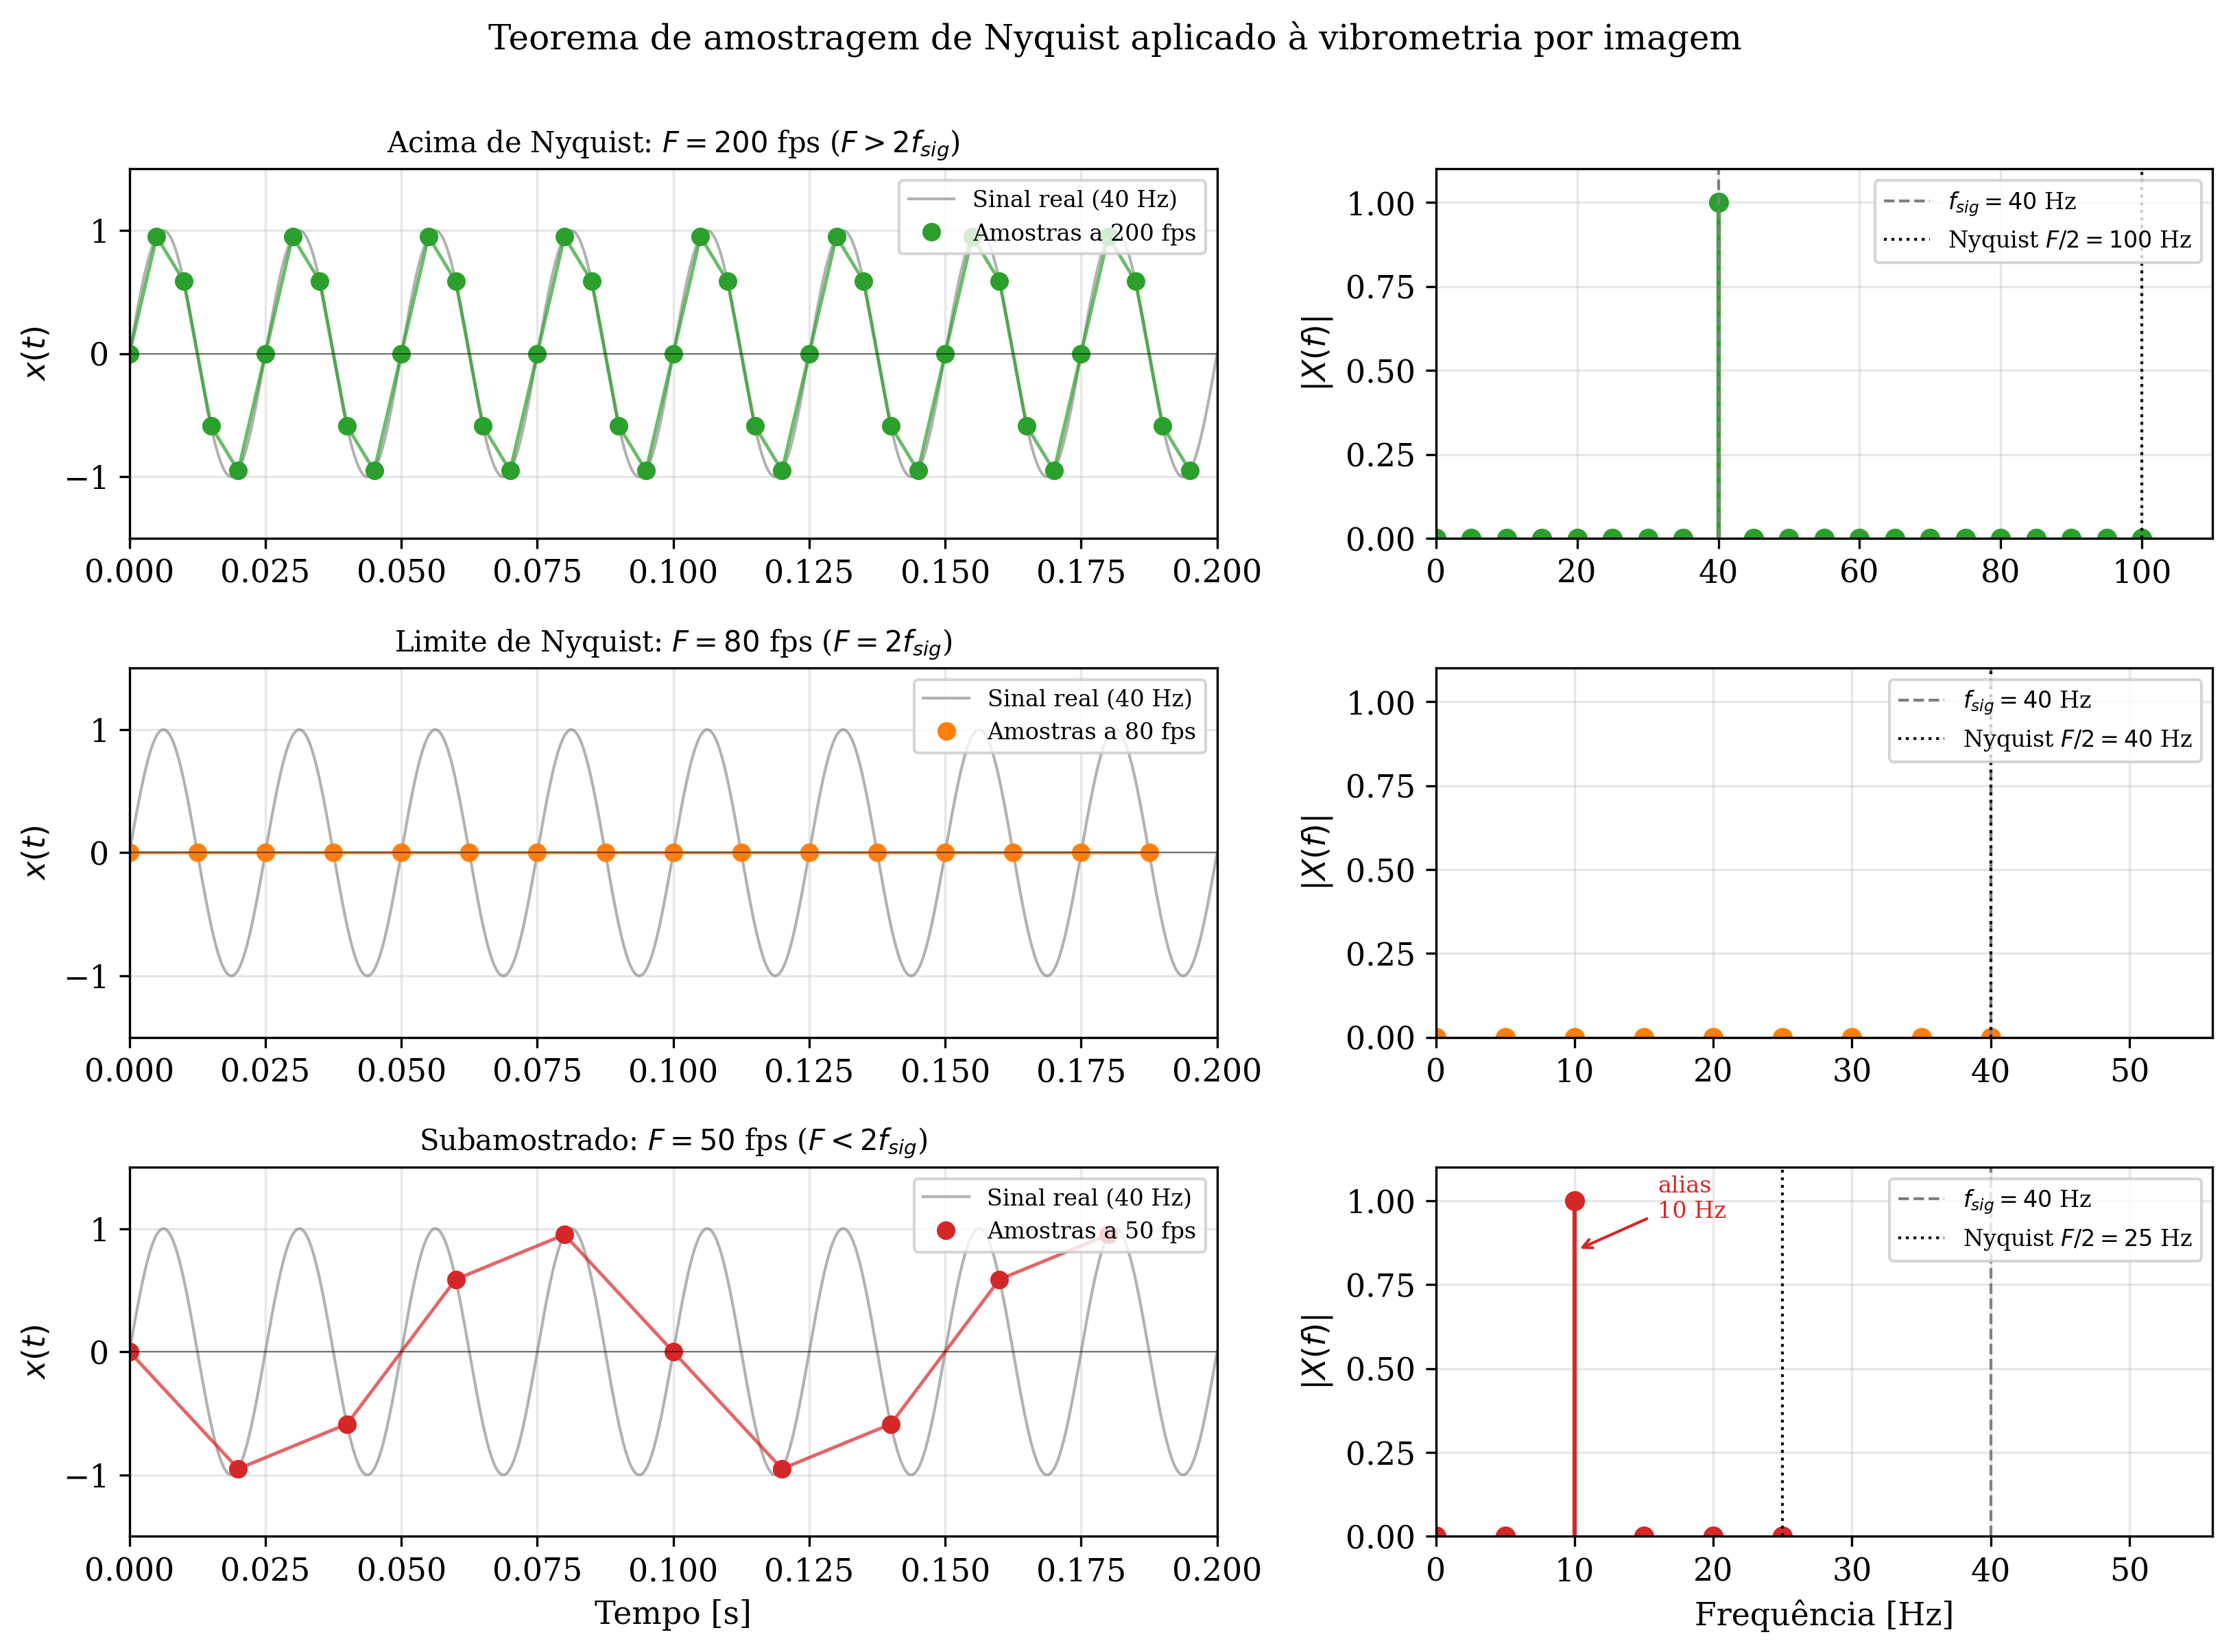
\includegraphics[width=\columnwidth]{Images/fig_nyquist_aliasing.png}
    \caption{Teorema de amostragem de Nyquist e efeito de aliasing. Fonte: O autor.}
    \label{fig:nyquist_aliasing}
\end{figure}

Dois parâmetros adicionais da câmera merecem atenção. O tempo de exposição deve ser curto o suficiente para que cada quadro registre o movimento como praticamente congelado; exposições longas introduzem borramento (\textit{motion blur}) que atenua artificialmente a amplitude medida \cite{LavatelliZappa2017}. A relação $\Delta x_{blur} \approx v \cdot t_{exp}$, em que $v$ é a velocidade instantânea do ponto e $t_{exp}$ o tempo de exposição, fornece uma estimativa direta desse efeito \cite{LavatelliZappa2017}. Já o tipo de obturador é crítico: o obturador global (\textit{global shutter}) captura todo o sensor simultaneamente, enquanto o obturador de rolagem (\textit{rolling shutter}) captura linha a linha, introduzindo distorções geométricas em vibrações rápidas. Para vibrometria, o obturador global é fortemente preferido \cite{robotcamera2025}.

\begin{figure}[htbp]
    \centering
    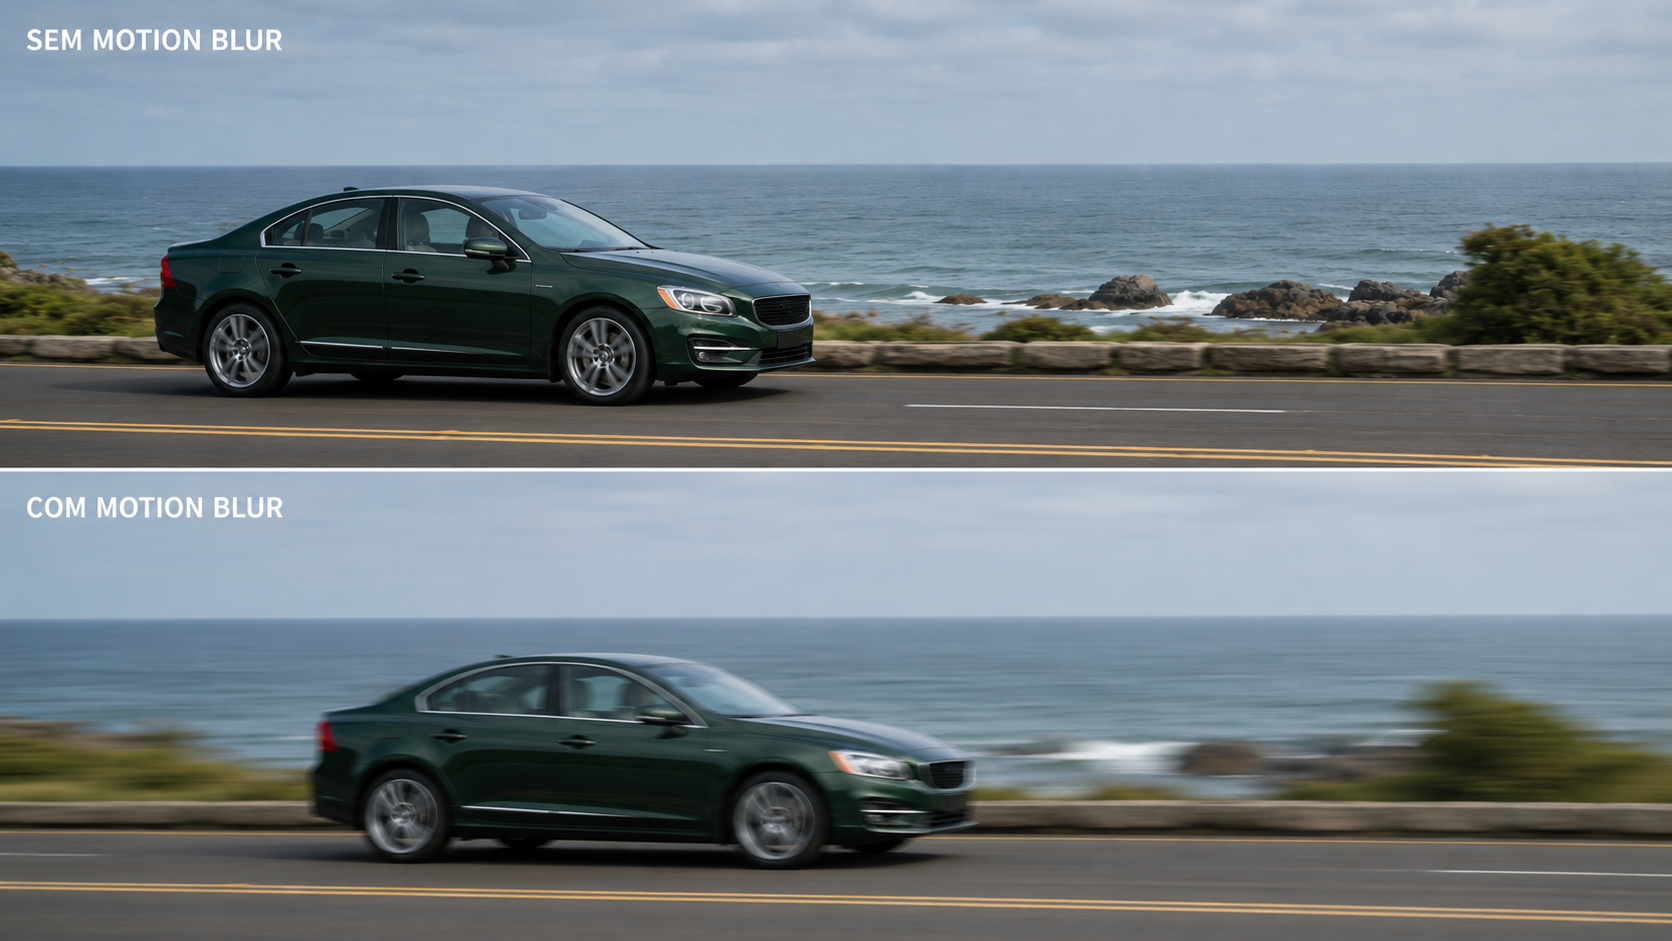
\includegraphics[width=\columnwidth]{Images/fig_motion_blur.png}
    \caption{Efeito de borramento por movimento. Fonte: O autor.}
    \label{fig:motion_blur}
\end{figure}

A calibração espacial converte deslocamentos medidos em pixels para unidades físicas (mm/pixel), tipicamente por meio de um objeto de referência de dimensões conhecidas posicionado no mesmo plano da peça. Em \cite{robotcamera2025}, por exemplo, foi obtida resolução espacial de 0,6~mm/pixel com câmera a 1,2~m da peça e lente de 20~mm de distância focal.

\subsubsection{Estimativa de movimento baseada em fase com filtros de Gabor}

O método central a ser implementado neste trabalho é a estimativa de movimento baseada em fase (\textit{Phase-Based Motion Estimation}, PME), obtida por meio da decomposição local da imagem com filtros de Gabor. Diferentemente de abordagens que operam diretamente sobre a intensidade dos pixels como o rastreamento por correspondência de padrões e o \textit{Digital Image Correlation} (DIC) clássico, a abordagem baseada em fase explora a propriedade fundamental de que, em uma vizinhança espacial estreita, pequenas translações de uma estrutura visual se manifestam como variações lineares na fase de coeficientes complexos obtidos por filtragem direcional \cite{Wadhwa2013, Phase2022}. Como a fase local é uma quantidade intrinsecamente robusta a variações de iluminação e a ruído da câmera, essa formulação alcança sensibilidades sub-pixel da ordem de milésimos de pixel, sem exigir marcadores artificiais nem padrões de \textit{speckle} aplicados à superfície \cite{ZhangLogGabor2024, WangLogGabor2022}.

O filtro de Gabor é um filtro de banda passante orientado, definido pelo produto de uma senoide complexa com uma envoltória gaussiana. Em duas dimensões, sua resposta ao impulso pode ser escrita, para uma orientação $\theta$ e uma frequência central $\omega_0$, como \cite{Wadhwa2013}:
\begin{equation}
    G_{\theta,\omega_0}(x,y) = \exp\!\left(-\frac{x'^{2} + y'^{2}}{2\sigma^{2}}\right) \cdot \exp\!\left(\, j\,\omega_0 \, x'\,\right),
    \label{eq:gabor_kernel}
\end{equation}
em que $(x', y') = (x\cos\theta + y\sin\theta,\; -x\sin\theta + y\cos\theta)$ são as coordenadas rotacionadas segundo $\theta$ e $\sigma$ controla a extensão espacial da envoltória gaussiana. A convolução do quadro $I(x,y,t)$ com $G_{\theta,\omega_0}$ produz um coeficiente complexo $C_{\theta,\omega_0}(x,y,t)$ em cada pixel:
\begin{equation}
    C_{\theta,\omega_0}(x,y,t) = \big(I * G_{\theta,\omega_0}\big)(x,y,t) = A(x,y,t)\,\exp\!\big(j\,\varphi(x,y,t)\big),
    \label{eq:gabor_coef}
\end{equation}
do qual se extraem dois mapas: a amplitude local $A = |C|$, que indica a presença de textura na orientação $\theta$ e frequência $\omega_0$, e a fase local $\varphi = \arg(C)$, que codifica a posição sub-pixel da estrutura naquela banda \cite{Wadhwa2013}.

A conexão entre fase e deslocamento é direta. Considere uma borda unidimensional descrita, em torno de um ponto, por uma senoide local de frequência espacial $\omega_0$. Se a borda se desloca uma quantidade $\delta(t)$ ao longo da direção perpendicular à orientação $\theta$, a variação da fase local entre dois quadros é dada por \cite{Wadhwa2013, Phase2022}:
\begin{equation}
    \Delta \varphi(x,y,t) = \varphi(x,y,t) - \varphi(x,y,t_0) \approx \omega_0 \, \delta(t),
    \label{eq:fase_deslocamento}
\end{equation}
de modo que o deslocamento na direção da fase é recuperado simplesmente por $\delta(t) \approx \Delta\varphi / \omega_0$. Essa relação é o núcleo da estimativa de movimento baseada em fase: o cálculo do deslocamento é reduzido a uma diferença de fases entre quadros, sem necessidade de busca explícita por correspondência de padrões \cite{Wadhwa2013}.

Para recuperar deslocamentos em direções arbitrárias e em diferentes escalas, aplica-se um banco de filtros de Gabor com múltiplas orientações $\theta_k$ e múltiplas frequências centrais $\omega_{0,\ell}$. As fases extraídas em cada par $(\theta_k, \omega_{0,\ell})$ fornecem componentes de deslocamento que, combinadas, permitem reconstruir o vetor $\vec{d}(x,y,t)$ de deslocamento em cada pixel \cite{Wadhwa2013}. Para uma região de interesse (ROI) definida no quadro de referência, o deslocamento médio é tipicamente obtido por uma média ponderada pela amplitude local $A$, dado que pixels de baixa amplitude carregam pouca informação confiável sobre a fase \cite{Phase2022, WangLogGabor2022}. Para suprimir movimentos espúrios da câmera ou do tripé, é prática comum incluir ao menos uma ROI fixada a um ponto rígido do fundo da cena, cujo deslocamento estimado é subtraído das demais ROIs como referência \cite{Mhatre2026, robotcamera2025}.

A grande vantagem dessa formulação para a vibrometria é a capacidade nativa de medição \textit{full-field} com alta sensibilidade: dado que a fase é avaliada em cada pixel, dezenas ou centenas de pontos podem ser monitorados simultaneamente no mesmo vídeo, simulando um arranjo virtual de sensores que seria proibitivo de implementar com acelerômetros físicos \cite{robotcamera2025}. Em comparação direta com métodos baseados em correlação de intensidade, a estimativa baseada em fase é menos sensível a ruído fotométrico e a pequenas variações de iluminação, e alcança sensibilidades reportadas da ordem de $0,003$~pixel em condições controladas \cite{ZhangLogGabor2024}. Como contraponto, a fase apresenta não-linearidades em regiões de baixa amplitude ou em padrões com componentes espectrais fora da banda do filtro, motivando a escolha cuidadosa dos parâmetros $(\omega_0, \sigma, \theta_k)$ e, em literatura mais recente, o uso de variantes como o filtro \textit{log-Gabor}, que elimina componente DC e oferece melhor cobertura espectral em superfícies pouco texturizadas \cite{WangLogGabor2022, ZhangLogGabor2024}.

\subsubsection{Análise espectral dos sinais de deslocamento}

Concluído o rastreamento, cada ROI produz dois sinais discretos no tempo, $x(t_k)$ e $y(t_k)$, amostrados à taxa $F$ da câmera. Esses sinais são equivalentes, do ponto de vista da análise dinâmica, aos sinais que seriam fornecidos por sensores de deslocamento posicionados em cada ROI. A análise dos sinais segue o procedimento clássico da análise vibracional experimental.

No domínio do tempo, a inspeção direta dos sinais permite identificar amplitudes, decaimentos exponenciais (com extração da razão de amortecimento $\zeta$ pelo decremento logarítmico) e correlação temporal entre diferentes pontos da estrutura. No domínio da frequência, a Transformada Rápida de Fourier (\textit{Fast Fourier Transform}, FFT) é aplicada para identificar as componentes espectrais dominantes, revelando as frequências naturais da peça e suas respectivas amplitudes modais \cite{Mhatre2026}.

Para ensaios em que a frequência de excitação varia ao longo do tempo (\textit{frequency sweeps}, partidas e paradas de máquinas), a Transformada de Fourier de Tempo Curto (\textit{Short-Time Fourier Transform}, STFT) é mais apropriada, pois fornece um espectrograma representação conjunta tempo-frequência que permite acompanhar a evolução das componentes espectrais ao longo do ensaio \cite{robotcamera2025}. Quando o sinal de excitação aplicado à base é conhecido (por exemplo, a partir de um acelerômetro montado no \textit{shaker}), pode-se ainda calcular a FRF experimental ponto a ponto como a razão entre o espectro de saída em cada ROI e o espectro de entrada na excitação, conforme aplicado em \cite{robotcamera2025} para identificação de ressonâncias estruturais em manipuladores robóticos.

\subsubsection{Desafios práticos e fontes de erro}

A vibrometria por imagem não está livre de limitações, e o desempenho do sistema depende de um conjunto de cuidados experimentais. Os principais desafios encontrados na literatura e a serem tratados neste trabalho são:

\begin{itemize}
    \item Iluminação: variações temporais na intensidade luminosa podem ser interpretadas pelo algoritmo de correspondência como movimento aparente. A solução é iluminação contínua e estável (LED de qualidade, evitando fontes com modulação PWM) e, quando necessário, pré-processamento dos quadros para normalização de intensidade \cite{robotcamera2025}.
    \item Movimento da câmera: qualquer vibração do tripé ou do suporte da câmera contamina todas as ROIs simultaneamente. A mitigação envolve fixação rígida do suporte e, como já mencionado, a subtração do movimento de uma ROI de referência fixada ao fundo \cite{Mhatre2026}.
    \item Limite de Nyquist e \textit{aliasing}: vibrações de frequência superior a $F/2$ produzem componentes espectrais espúrias. Esse limite define a escolha da câmera para a aplicação pretendida; em \cite{robotcamera2025}, por exemplo, uma câmera a 1000~fps permitiu análise confiável até cerca de 125~Hz.
    \item Textura da superfície: regiões de baixa textura (superfícies lisas e uniformes) produzem amplitude local $A$ próxima de zero na saída do filtro de Gabor, tornando a fase indefinida e contaminando a estimativa de deslocamento. Quando a textura natural da peça é insuficiente, pode-se recorrer à aplicação de um \textit{speckle pattern} artificial ou de marcadores de alto contraste em pontos de medição específicos \cite{robotcamera2025, Mhatre2026}.
    \item Custo computacional: a aplicação de um banco de filtros de Gabor com múltiplas orientações e escalas a cada quadro de um vídeo longo em alta resolução é computacionalmente exigente. As estratégias usuais incluem a restrição do processamento às ROIs de interesse, a implementação das convoluções no domínio da frequência via FFT, e a paralelização em GPU quando disponível \cite{robotcamera2025}.
\end{itemize}

Mesmo com esses cuidados, a vibrometria por imagem não substitui integralmente os métodos tradicionais. Ela se posiciona como um complemento de alto valor, particularmente em cenários em que o \textit{mass loading} é proibitivo, em que o número de pontos de medição desejado é grande, ou em que se busca informação espacial de modos de vibrar para fins de SHM e análise forense de falhas.

\section{Metodologia}

Com o objetivo de validação de hipóteses, a abordagem realizada começou na criação de um Produto Mínimo Viável e, em sequência, evoluiu para um sistema mais robusto.

\subsection{Produto Mínimo Viável (MVP)}

O MVP segue três pilares principais: Viabilidade, Valor e Capacidade de Aprendizado, seguindo os princípios de reduzir riscos, agilidade e foco no essencial.

Com o objetivo de simular a oscilação de 1~GDL de uma viga engastada (\textit{cantilever}) validando a aquisição de dados a partir desse movimento, foram selecionados os seguintes equipamentos:

\begin{itemize}
    \item Câmera DJI Osmo Action 4;
    \item Régua com marcador na ponta;
    \item Bancada para teste.
\end{itemize}

\subsection{Equipamentos Utilizados}

\subsubsection{Câmera de aquisição}

A câmera selecionada para os ensaios é a DJI Osmo Action 4, equipada com sensor CMOS de 1/1{,}7'' e abertura fixa de $f$/2{,}8. Para as finalidades de vibrometria, os modos de captura relevantes são 4K a 120\,fps e 1080p a 240\,fps, que estabelecem frequências de Nyquist de, respectivamente, 60\,Hz e 120\,Hz. O modo de 240\,fps é preferido sempre que a frequência fundamental da estrutura sob análise estiver abaixo de 100\,Hz, satisfazendo a recomendação prática de operar com taxa de captura ao menos cinco vezes superior à frequência máxima de interesse \cite{robotcamera2025}.

O sensor da câmera opera com obturador de rolagem (\textit{rolling shutter}), capturando o sensor linha a linha ao invés de instantaneamente. Em oscilações de amplitude elevada, esse mecanismo introduz distorções geométricas entre linhas consecutivas do quadro \cite{robotcamera2025}, constituindo uma limitação relevante para a vibrometria por imagem. A mitigação é realizada mantendo o tempo de exposição suficientemente curto (tipicamente $t_{exp} \leq 1/2000\,\text{s}$), de modo que o deslocamento da estrutura durante cada quadro seja desprezível frente à amplitude total da vibração \cite{LavatelliZappa2017}. A função de estabilização eletrônica RockSteady é desativada durante todos os ensaios, uma vez que esse recurso altera artificialmente o conteúdo de movimento do vídeo e comprometeria a extração de fase.

\subsubsection{Estrutura vibratória e bancada}

A estrutura de teste é uma régua graduada fixada por grampo em uma das extremidades, simulando uma viga engastada-livre (\textit{cantilever}). Esse modelo é escolhido por representar, de forma controlada e analiticamente tratável, o comportamento de 1~GDL de interesse. Na extremidade livre, é aplicado um marcador de alto contraste --- ponto preto sobre fundo branco --- que eleva a amplitude local $A$ na saída dos filtros de Gabor, tornando a estimativa de fase mais confiável naquela região de interesse \cite{Wadhwa2013}. O comprimento livre $L$, a largura $b$ e a espessura $h$ da régua são medidos antes de cada ensaio para alimentar o modelo analítico descrito na Seção~\ref{sec:modelagem}.

A bancada de suporte consiste em uma mesa rígida sobre a qual o grampo é fixado. Uma região estática da bancada é designada como ROI de referência, cujo sinal de deslocamento estimado é subtraído das demais ROIs de medição para compensar eventuais vibrações de corpo rígido da câmera ou do suporte \cite{Mhatre2026}.

A calibração espacial é realizada com um objeto de referência de dimensões conhecidas posicionado no plano focal da câmera, imediatamente antes de cada sessão de ensaio. O fator de escala $s$ [mm/pixel] é extraído da razão entre a dimensão física conhecida e o número de pixels correspondente na imagem, sendo utilizado para converter os deslocamentos estimados pelo algoritmo de pixel para milímetro.

\subsection{Modelagem e Simulação}
\label{sec:modelagem}

\subsubsection{Modelo analítico da viga cantilever}

A régua é modelada como uma viga de Euler-Bernoulli com seção retangular uniforme de largura $b$ e espessura $h$. Para o primeiro modo de flexão de uma viga engastada-livre, a frequência natural é \cite{Rao2010}:

\begin{equation}
    f_{n,1} = \frac{(\beta_1 L)^2}{2\pi L^2}\sqrt{\frac{EI}{\rho A}},
    \label{eq:fn_cantilever}
\end{equation}

em que $\beta_1 L = 1{,}8751$ é a raiz característica do primeiro modo, $I = bh^3/12$ é o momento de inércia de área, $A = bh$ é a área da seção transversal, $E$ é o módulo de Young e $\rho$ é a densidade do material. Substituindo $I$ e $A$, a Equação~\ref{eq:fn_cantilever} se simplifica para:

\begin{equation}
    f_{n,1} = \frac{(1{,}8751)^2\, h}{2\pi\sqrt{12}\, L^2}\sqrt{\frac{E}{\rho}},
    \label{eq:fn_simplificado}
\end{equation}

evidenciando que $f_{n,1}$ é proporcional à espessura $h$ e inversamente proporcional a $L^2$, o que permite ajustar a frequência do ensaio simplesmente variando o comprimento livre encastrado. Para o cálculo da resposta temporal, a viga é reduzida a um sistema de 1~GDL com parâmetros equivalentes avaliados na ponta livre \cite{Rao2010, Downey2026}:

\begin{equation}
    k_{eq} = \frac{3EI}{L^3}, \qquad m_{eq} = 0{,}2357\,\rho A L.
    \label{eq:keq_meq}
\end{equation}

A Tabela~\ref{tab:parametros_materiais} apresenta os parâmetros dos materiais mais comuns em réguas de escritório, utilizados como estimativa inicial de $f_{n,1}$ antes da medição geométrica da régua real.

\begin{table}[htbp]
    \centering
    \caption{Parâmetros materiais de referência para estimativa de $f_{n,1}$.}
    \label{tab:parametros_materiais}
    \small
    \begin{tabularx}{\columnwidth}{l c c}
        \toprule
        \textbf{Material} & \textbf{$E$ (GPa)} & \textbf{$\rho$ (kg/m\textsuperscript{3})} \\
        \midrule
        Aço inox      & 193 & 7850 \\
        Polipropileno & 1{,}5 & 900 \\
        \bottomrule
    \end{tabularx}
\end{table}

\subsection{Resultados Preliminares}



\section{Resultados e Discussão}

\section{Considerações Finais}

%==============================================================================
%  REFERENCIAS 
%==============================================================================
\bibliographystyle{unsrt}
\bibliography{referencias}

\end{document}